\documentclass[12pt,a4paper,twoside]{scrartcl}
\usepackage[english,ngerman]{babel}
\usepackage[T1]{fontenc}
\usepackage{lmodern}
\usepackage[utf8]{inputenc}
\usepackage[tmargin=22mm,bmargin=22mm,lmargin=20mm,rmargin=20mm]{geometry}
\usepackage{latexsym,amsmath,amssymb,mathtools,textcomp}
\usepackage{parskip}
\usepackage{amsthm}
\usepackage{bbm}
\usepackage{mathtools}
\usepackage{indentfirst}
\usepackage{setspace}
\usepackage{csquotes}
\usepackage{titlesec}
\begingroup
\makeatletter
\@for\theoremstyle:=definition,remark,plain\do{%
  \expandafter\g@addto@macro\csname th@\theoremstyle\endcsname{%
    \addtolength\thm@preskip\parskip
  }%
}
\endgroup

\newtheorem{theorem}{Theorem}[section]
\newtheorem{definition}[theorem]{Definition}
\newtheorem{lemma}[theorem]{Lemma}

\numberwithin{equation}{section}
\DeclareOldFontCommand{\bf}{\normalfont\bfseries}{\mathbf}

\usepackage{graphicx}
\graphicspath{{images/}}
\usepackage{array,multirow}
\usepackage{enumitem}
\setlist[enumerate]{topsep=0pt}
\setlist[itemize]{topsep=0pt}
\setlist[description]{font=\normalfont,topsep=0pt}

\titleclass{\subsubsubsection}{straight}[\subsection]

\newcounter{subsubsubsection}[subsubsection]
\renewcommand\thesubsubsubsection{\thesubsubsection.\arabic{subsubsubsection}}
\renewcommand\theparagraph{\thesubsubsubsection.\arabic{paragraph}} % optional; useful if paragraphs are to be numbered

\titleformat{\subsubsubsection}
  {\normalfont\normalsize\bfseries}{\thesubsubsubsection}{1em}{}
\titlespacing*{\subsubsubsection}
{0pt}{3.25ex plus 1ex minus .2ex}{1.5ex plus .2ex}

\makeatletter
\renewcommand\paragraph{\@startsection{paragraph}{5}{\z@}%
  {3.25ex \@plus1ex \@minus.2ex}%
  {-1em}%
  {\normalfont\normalsize\bfseries}}
\renewcommand\subparagraph{\@startsection{subparagraph}{6}{\parindent}%
  {3.25ex \@plus1ex \@minus .2ex}%
  {-1em}%
  {\normalfont\normalsize\bfseries}}
\def\toclevel@subsubsubsection{4}
\def\toclevel@paragraph{5}
\def\toclevel@paragraph{6}
\def\l@subsubsubsection{\@dottedtocline{4}{7em}{4em}}
\def\l@paragraph{\@dottedtocline{5}{10em}{5em}}
\def\l@subparagraph{\@dottedtocline{6}{14em}{6em}}
\makeatother

\setcounter{secnumdepth}{4}
\setcounter{tocdepth}{4}


\usepackage{float}
\usepackage{tikz}
\usetikzlibrary{calc}
\usepackage{fancyhdr}
\fancypagestyle{plain}{
  \setlength\footskip{32pt}
  \fancyhead{}
  \fancyfoot{}
  \fancyfoot[LE,RO]{\normalsize\thepage}
  \renewcommand{\headrulewidth}{0pt}
  \renewcommand{\footrulewidth}{0pt}
}

\usepackage{ctable}
\fancypagestyle{normal}{
  \setlength{\headheight}{20pt}
  \setlength\footskip{32pt}
  \fancyhead{}
  \fancyhead[LE]{\normalsize\textsc{\nouppercase{\leftmark}}}
  \fancyhead[RO]{\normalsize\textsc{\nouppercase{\rightmark}}}
  \fancyfoot{}
  \fancyfoot[LE,RO]{\normalsize\thepage}
  \renewcommand{\headrulewidth}{0.4pt}
  \renewcommand{\footrulewidth}{0pt}
}

\usepackage{color}
\usepackage[pagebackref]{hyperref}
\usepackage[all]{hypcap}
\usepackage{cleveref}
\usepackage[font=small,belowskip=6pt]{subcaption}
\usepackage[section]{placeins}

\usepackage[titletoc,toc,title,page]{appendix}
\usepackage{pdfpages}
\usepackage[export]{adjustbox}

\usepackage{pgfplots}
\usepackage{tikz}
\usepackage{lmodern}
\usepackage{multirow}
\usepackage{makecell}
\usepackage{boldline}
\usepackage{array}
\usepackage{caption}
\usepackage{varwidth}
\usepackage{threeparttablex}
\usepackage{rotating}


\hypersetup{
  pdftitle={Automatische Auswahl von maschinellen Lernverfahren für kausale Inferenz},
  pdfauthor={Atanas Dimitrov}, 
  pdfsubject={causal inference,synth validation, machine learning, gradient boosting, lasso, causal forest}
  colorlinks=true,
  pdfborder={0 0 0},
  bookmarksopen=true,
  bookmarksopenlevel=1,
  bookmarksnumbered=true,
  linkcolor=blue!60!black,
  % linkcolor=black,
  citecolor=blue!60!black,
  urlcolor=blue!60!black,
  filecolor=green!60!black,
  pdfpagemode=UseNone,
  unicode=true,
}
\renewcommand{\appendixpagename}{\appendixname} 
\renewcommand{\appendixtocname}{\appendixname}

\renewcommand{\baselinestretch}{1.2} 
\renewcommand*{\backreflastsep}{, }
\renewcommand*{\backreftwosep}{, }
\renewcommand*{\backref}[1]{}
\renewcommand*{\backrefalt}[4]{%
  \ifcase #1 %
  Keine Zitierungen.
  \or
  (Seite #2).%
  \else
  (Seiten #2).%
  \fi%
}
\usepackage{import}

\newcommand\independent{\protect\mathpalette{\protect\independenT}{\perp}}
\def\independenT#1#2{\mathrel{\rlap{$#1#2$}\mkern2mu{#1#2}}}

\newcommand{\reffig}[1]{\emph{\hyperref[#1]{Abbildung \ref*{#1}}}}
\newcommand{\refsec}[1]{\emph{\hyperref[#1]{Abschnitt \ref*{#1} }}}
\newcommand{\refapp}[1]{\emph{\hyperref[#1]{Anhang \ref*{#1}}}}

\renewcommand*{\refeq}[1]{\emph{\hyperref[#1]{Gleichung \ref*{#1} }}}

\renewcommand\theadalign{bc}
\renewcommand\theadfont{\bfseries}
\renewcommand\theadgape{\Gape[4pt]}
\renewcommand\cellgape{\Gape[4pt]}

\newcolumntype{L}[1]{>{\raggedright\let\newline\\\arraybackslash\hspace{0pt}}m{#1}}
\newcolumntype{C}[1]{>{\centering\let\newline\\\arraybackslash\hspace{0pt}}m{#1}}
\newcolumntype{R}[1]{>{\raggedleft\let\newline\\\arraybackslash\hspace{0pt}}m{#1}}



\newcounter{mypagecount}% create a new counter
\setcounter{mypagecount}{0}% set it to something just in case
\newenvironment{interlude}{% create a new environment for the unnumbered section(s)
  \clearpage
  \setcounter{mypagecount}{\value{page}}% use the new counter we created to hold the page count at the start of the unnumbered section
  \thispagestyle{empty}% we want this page to be empty (adjust to use a modified page style)
  \pagestyle{empty}% use the same style for subsequent pages in the unnumbered section
}{%
  \clearpage
  \setcounter{page}{\value{mypagecount}}% restore the incremented value to the official tally of pages so the page numbering continues correctly
}

% Package for inserting pseudo codes in the document.
\usepackage[ruled,vlined,linesnumbered,norelsize]{algorithm2e}
\DontPrintSemicolon
\def\NlSty#1{\textnormal{\fontsize{8}{10}\selectfont{}#1}}
\SetKwSty{texttt}
\SetCommentSty{emph}
\def\listalgorithmcfname{List of Algorithms}
\def\algorithmautorefname{Algorithm}
\let\chapter=\section % resolve a problem with algorithm2


\begin{document}
\boldmath
\nonfrenchspacing

\pagestyle{empty}
\pagenumbering{alph}


\setlength{\parindent}{4em}
\setlength{\parskip}{1em}

% title page
\begin{titlepage}

  \begin{center}\large

    {\flushleft
\includegraphics[height=17mm, width=45mm]{kit_logo_en.pdf} \hfill}
    
\includegraphics[height=15mm, width=45mm]{group_logo.pdf}\quad\null

    \vspace*{1cm}
    {\Large Bachelorarbeit}\\
    \noindent\hfil\rule{0.4\textwidth}{.4pt}\hfil
    \vspace*{1cm}

    {\bf\huge Automatische Auswahl von maschinellen Lernverfahren für kausale Inferenz\par}
    \vspace*{5mm}

    von\\
    \vspace*{3mm}
    {\huge{Atanas Dimitrov}}

    \vspace*{10mm}
    Pervasive Computing Systems / TECO\\
    Institut für Telematik\\
	Fakultät für Informatik\\
   
    \vspace*{15mm}

   	Abgabadatum: 02.09.2019 %TODO
    \vspace*{10mm}


    \begin{tabular}{p{8cm}l}
     Verantwortlicher Betreuer: &Prof. Dr. Michael Beigl\\
     Betreuerin: &Ployplearn Ravivanpong\\  
    \end{tabular}

    \vspace*{8mm}

  \end{center}

\end{titlepage}

\selectlanguage{ngerman}

\centerline{\bf\large Erklärung}

\vspace*{12mm}

{\setstretch{1.5}\large Hiermit erkläre ich, dass ich die vorliegende Bachelorarbeit selbstständig verfasst und keine anderen als die angegebenen Hilfsmittel und Quellen benutzt habe, die wörtlich oder inhaltlich übernommenen Stellen als solche kenntlich gemacht und weiterhin die Richtlinien des KIT zur Sicherung guter wissenschaftlicher Praxis beachtet habe.\par}

\vfill
\noindent
{\large Karlsruhe, 02.09.2019}
\hrule


\vspace*{5cm}

\clearpage

%%%%%%%%%%%%%%%%%%%%%%%%%%%%%%%%%%%%%%%%%%%%%%%%%%%%%%%%%%%%%%%%%%%%%% 

\vspace*{0pt}\vfill

\selectlanguage{ngerman}

\begin{abstract}
  \centerline{\bf Abstract}
  \vspace*{1cm}
 Diese Bachelorarbeit beschäftigt sich mit dem Vergleich von Methoden für kausale Inferenz und mit der automatischen Auswahl von dem besten von denen abhängig von dem vorhandenen Datensatz. Dazu benutzen und erweitern wir Synth-Validation - ein Verfahren, mit dem von den echten Daten synthetische Daten mit einem gewünschtem durchschnittlichen Behandlungseffekt erstellt und dann ausgewertet werden. Dabei haben die Datensätze, auf denen wir unsere Experimente durchführen, unterschiedliche Natur - echten Rohdaten mit größeren oder kleineren Zahl von Kovariaten, von Rohdaten synthetisch generierten Daten und zufällig generierten Daten. Die kausale Inferenz Verfahren, von denen Synth-Validation auswählt, benutzen ausschließlich Algorithmen aus dem maschinellem Lernen. Es wird die Fähigkeit von Synth-Validation gemessen, den Verfahren zu wählen, der die nächste Schätzung von dem durchschnittlichen Behandlungseffekt hat. Das wird unter unterschiedlichen Konstellationen unterstellt - nach der Art der Daten, nach der Anzahl der Elementen in der Stichprobe usw.          
\end{abstract}

\vfill\vfill\vfill
\clearpage

%%%%%%%%%%%%%%%%%%%%%%%%%%%%%%%%%%%%%%%%%%%%%%%%%%%%%%%%%%%%%%%%%%%%%% 
\selectlanguage{ngerman}
\pagestyle{plain}
\pagenumbering{roman}

% markiere sections im Seitenkopf links und subsections rechts
\renewcommand\sectionmark[1]{\markboth{\thesection\quad\MakeUppercase{#1}}{\thesection\quad\MakeUppercase{#1}}}
\renewcommand\subsectionmark[1]{\markright{\thesubsection\quad\MakeUppercase{#1}}}

\tableofcontents
\clearpage
%%%%%%%%%%%%%%%%%%%%%%%%%%%%%%%%%%%%%%%%%%%%%%%%%%%%%%%%%%%%%%%%%%%%%% 
\listoffigures
\clearpage

\pagestyle{normal}
\pagenumbering{arabic}

%main content starts here
\nocite{*} %TODO remove when all references ready 
\section{Einführung}\label{sec:einführung}
Um die Welt besser zu verstehen, haben die Menschen immer die Antwort auf der folgenden Frage gesucht: Was passiert, wenn eine bestimmte Tat oder Handlung durchgeführt wird? Manche Handlungen kann man als \enquote{einfach} qualifizieren und bei denen ist diese Antwort leicht zu erreichen. Wenn man einen Apfel nach oben wirft, fällt er wieder nach unten. Es kostet (fast) nichts, diese Tatsache zu prüfen. Fast jeder kann dieses Ergebnis vorhersagen, weil man irgendwann mal ein fallendes Objekt beobachtet hat, unabhängig davon, ob man weiß, warum die Objekte fallen. Handlungen können aber deutlich komplexer sein wie z.B. Einnahme einer neuen Steuerpolitik oder die medizinische Behandlung mit einem Medikamenten. Diese Handlungen sind schwerer durchzuführen, sind von mehreren Faktoren oder Naturgesetzen betroffen, sind \enquote{abhängiger}. Auf Basis früherer Erfahrung im Bereich können Experten Rahmen davon setzen, was passieren wird. Sicher kann man nur dann sein, wenn die Handlung durchführt ist und man beobachtet und bemesst, was passiert hat. Die letzte Schlussfolgerung gilt sowohl für die \enquote{einfacheren}, als auch für die \enquote{komplexeren} Handlungen. Also um eine sichere Kenntnis zu erschaffen, brauchen wir Erfahrung - in dem Fall mit dem Apfel entweder werfen wir den alleine oder beobachten wir jemanden, der das macht oder der das irgendwann mal gemacht hat. Bei den \enquote{komplexeren} Handlungen ist meistens die Antwort auf der Frage \enquote{Was?}  nicht ausreichend - man braucht \enquote{Wie viel?}. Das führt uns langsam zu dem Sachverhalt der kausalen Inferenz.      
  	\subsection{Kausale Inferenz}\label{subsec:kausalität}
  	Wenn wir über die Kausalität in ihrem wissenschaftlichen Sinn sprechen, muss es klar sein, dass \enquote{\textbf{\textit{A}} verursacht \textbf{\textit{B}}} nicht bedeutet, dass \textbf{\textit{A}} der Hauptgrund ist, warum \textbf{\textit{B}} passiert hat. Es bedeutet, dass \textbf{\textit{A}} den Unterschied oder die Differenz gemacht hat, die zu \textbf{\textit{B}} geführt haben. Es existieren möglicherweise noch weitere Gründe z.B. \textbf{\textit{C}} und \textbf{\textit{D}}, ohne deren Existenz und ohne deren verursachten Differenz \textbf{\textit{B}} nicht möglich war oder nicht den Wert halten würde, den es hält. \textbf{\textit{A}} soll man nicht als eine Zuschreibung von \textbf{\textit{B}} anschauen, sondern als einen Beitrag\cite{MacHum}.  Dabei sollen wir unter \textbf{kausale Inferenz} ähnlich wie bei der statistischen Inferenz den Prozess und die Methodiken zum Finden von Kenntnissen über die Kausalität von irgendeiner Handlung, insbesondere das Finden von der Differenz, die sie verursacht.\par
  	

\noindent	
Die kausale Inferenz hat aber ein fundamentales Problem. Wenn wir den Effekt von einer Handlung wissen wollen, führen wir diese Handlung aus und bemessen den Wert von irgendeine Variable, die uns interessiert. Der echte Effekt ist aber die Differenz zwischen dieser Variable bedingt, dass wir die Handlung durchgeführt haben und die gleiche Variable, bedingt, dass wir die Handlung nicht durchgeführt haben\cite{holland1986statistics}. Natürlich ist nur eine der beiden Optionen direkt beobachtbar. Formal kann man es so dargestellt: \par
  	
\begin{equation}
  TE = (Y|W = 1) - (Y|W = 0)
\end{equation}  	
  	
\noindent	  	
Hier bezeichnet \textbf{\textit{TE}} das Behandlungseffekt, \textbf{\textit{Y}} ist die beobachtete Variable und \textbf{\textit{W}} ist eine binäre Variable, die bezeichnet, ob die Handlung durchgeführt wurde oder nicht.\par

\noindent	  	
Obwohl wir den Behandlungseffekt von einer Handlung individuell nicht beobachten können, können wir schätzen, wie hoch durchschnittlich diesen Effekt ist, wenn wir die Handlung auf mehreren Objekten durchführen beziehungsweise auch auf mehreren nicht durchführen und die Differenz zwischen diesen beiden Ergebnissen als \textbf{durchschnittliches Behandlungseffekt} oder auf Englisch \textbf{average treatment effekt(ATE)} bezeichnen. Meistens können wir die Behandlung nicht auf allen (oder eigentlich auf der Hälfte von allen) Objekten durchführen, sondern müssen wir eine Stichprobe ziehen.  Formal stellen wir das so dar: \par

\begin{equation}\label{eq:1.2}
  \tau = E_Y[Y|W = 1] - E_Y[Y|W = 0]
\end{equation}

\noindent
In dieser Modelldarstellung sind $W$ und $Y$ Zufallsvariablen. $W$ ist binär, wo \textbf{1} für eine Behandlung und \textbf{0} für keine Behandlung steht. $Y$ ist die Zufallsvariable von einem gewünschten Wert nach der potenziellen Behandlung. $E_Y$ steht für den Erwartungswert von \textbf{Y}. Schon in dieser Darstellung treffen wir allen Problemen, die man sonst in der statistischen Inferenz trifft - damit unsere Schätzung über die Stichprobe näher zu der echten ATE der Gesamtpopulation liegt, müssen bestimmte Regeln eingehalten werden.\par

\noindent
\refeq{eq:1.2} ist immer noch kein gutes Model der Wirklichkeit, weil es oft der Fall ist, dass die Objekten, die wir behandeln, sich durch einigen Merkmalen unterscheiden. Diese andere Differenzen können Einfluss auf $Y$ sowohl bedingt $W$, als auch unbedingt $W$ haben und diese Tatsache soll in der Gleichung einbezogen werden:\par

\begin{equation}\label{eq:1.3}
  \tau = E_{Y,X}[Y|X,W = 1] - E_{Y,X}[Y|X,W = 0]
\end{equation}       	

\noindent 
$X$ ist eine Zufallsvariable für die so genannten \textbf{Kovariaten}. $X$ ist mehrdimensional und stellt den Zustand, in dem sich ein Objekt oder allgemeiner gesagt eine Welt befindet. Die Kovariaten sollen nicht, aber können einen Einfluss auf das Ergebnis $Y$ haben. Diejenigen mit Einfluss nennen wir \textbf{Confounders} oder \textbf{confounding Variablen}. Auf Deutsch kann man den Begriff am nächsten mit dem Wort Verwirrungsvariablen übersetzen. Die Existenz von Confounders erschwert unsere Aufgabe, den Effekt zu finden, den die Behandlung verursacht.\cite{vanderweele2013definition}. \par

\noindent
In der Tat können Confounders auch indirekten Einfluss auf die Behandlung haben. Beispiel: Sei $X$ das Alter sein, $W$ - ob man raucht oder nicht und $Y$ - eine Gesundheitsmaß. Es ist klar, dass das Alter an sich einen Effekt auf der Gesundheit hat. Die empirische Daten zeigen aber auch, dass das Rauchen unter älteren Menschen verbreiteter ist als unter jüngeren, d.h das Alter bewirkt sowohl das Rauchen, als auch die Gesundheit, die an sich vom Rauchen bewirkt wird. Diese Abhängigkeiten werden in \reffig{fig:confounder} veranschaulicht.\par   	
\begin{center}
  \vspace{6mm}
  \begin{figure}[h]
    \centering
    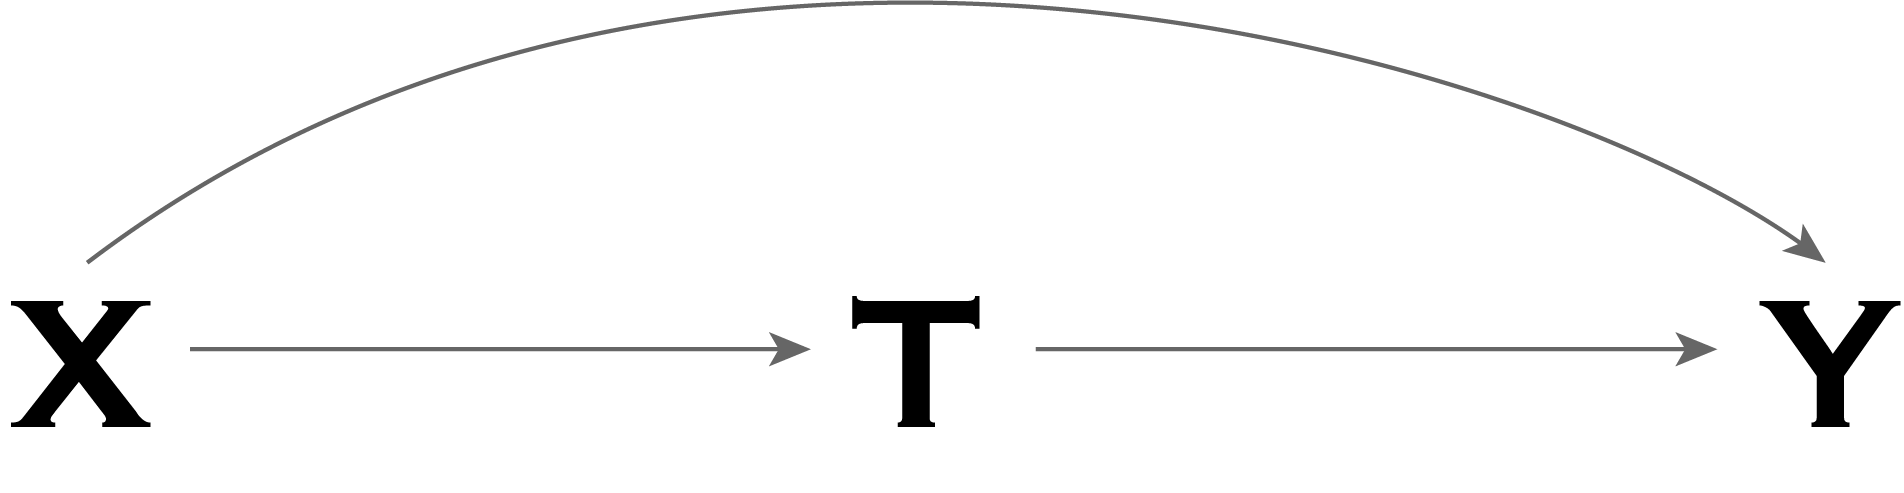
\includegraphics[height=0.4\textwidth, width=0.9\textwidth]{figures/confounder.png}
    \caption[Einfluss von Confounder auf Behandlung und Ergebnis]{Einfluss von Confounder auf Behandlung und Ergebnis\cite{RebBar}. Hier ist $X$ der Confounder, $T$ - die Behandlung und $Y$ - das Ergebnis. Es wird gezeigt, dass das Ergebniss nicht nur von der Behandlung abhängt, sondern auch vom Confounder. Der Confouder hat auch eine Auswirkung auf die Behandlung.}\label{fig:confounder}
  \end{figure}
\end{center}

\noindent
Wir schließen diesen Abschnitt mit der Gedanke von dem Philosophen David Lewis über die Kausalität, der sie folgendermaßen beschreibt: \enquote{etwas, was einen Unterschied verursacht und der Unterschied, den dieses etwas verursacht, soll der Unterschied  davon sein, was ohne dieses etwas passieren würde} \cite{lewis1974causation}.\par

\subsection{Motivation}\label{subsec:motivation}
Es ist wichtig zu wissen, was genau eine Handlung verursacht oder welche Differenz sie macht. Mit diesen Kenntnissen können wir besser die passenden Handlungen und deren genauen Maßen zum Erreichen unseres Ziels einschätzen und dann auswählen. Diese Behauptungen sind allgemeingültig und wir betrachten konkret drei Beispiele von unterschiedlichen Bereichen, wo das Kennen von dem durchschnittlichen Behandlungseffekt von großer Bedeutung ist.\par

\noindent
\textbf{Beispiel 1}\phantomsection\label{motivationBeispiel1} In der Pharmazie spielt die Kausalität eine besonders große Rolle. Wenn man einen Medikamenten entwickelt, soll man ganz genau wissen, welchen durchschnittlichen Effekt dieses Medikament auf unterschiedenen variablen körperlichen Werten hat - sowohl für wohltuende, als auch für schädliche Effekte. Hier ist das Nutzen, das die kausale Inferenz bringt, die Gesundheit der Menschen.\par

\noindent
\textbf{Beispiel 2}\phantomsection\label{motivationBeispiel2} Weitere Bedeutung hat die kausale Inferenz im Marketing und in der Bewertung von Werbungen. Eine Werbung kann eine Kette von unterschiedlichen Zielen haben, aber am Ende steht die Erhöhung von tatsächlichen Einkäufen von dem geworbenen Produkt oder Dienstleistung. Natürlich ist die Werbung nicht der einzige Treiber des Umsatzes. Also man muss nur den Effekt der Werbung einschätzen. Dann abhängig von diesem durchschnittlichen Effekt und dem Preis der Werbung stellt man fest, ob eine Werbung Nutzen bringt bzw. welche Werbung am nützlichsten ist.\par

\noindent
\textbf{Beispiel 3}\phantomsection\label{motivationBeispiel3} Die kausale Inferenz ist bedeutend für die Auswahl vom eigenen Verhalten sein. Zum Beispiel kann man den Einfluss vom regelmäßigen Rauchen von Rauschgift auf die mentalen Fähigkeiten untersuchen. Wenn man diesen durchschnittlichen Effekt kennt, sollte es wahrscheinlicher sein, dass man auf diese schlechte Sucht verzichtet oder am besten gar nicht damit anfängt. Diese deutliche wissenschaftliche Daten können durch den Gesetzgeber als Rechtfertigung für einen Verbot von diesem Stoff benutzt werden.\par
\subsection{Finden von ATE}\label{subsec:findenATE}
\noindent
\textit{Wir gehen davon aus, dass unser Problem schon klar definiert ist: Welchen durchschnittlichen Effekt(ATE) verursacht eine Behandlung? In diesem Abschnitt erläutern wir, wie man genau mit diesem Problem in den unterschiedlichen Situationen umgeht.}\par

\vspace{7mm}

Grundsätzlich muss man \refeq{eq:1.3} lösen, die wir zur Bequemlichkeit hier noch mal hinbringen.\par 

\begin{equation}\label{eq:1.4}
  \tau = E_{Y,X}[Y|X,W = 1] - E_{Y,X}[Y|X,W = 0]
\end{equation}  

\noindent
Dazu gibt es zwei Vorgehensweisen, die sich durch die Art von Datensammlung unterscheiden - Durchführung von einem Experimenten und Durchführung von einer Beobachtungsstudie. Die Daten aus den unterschiedlichen Studien wertet man dann anders aus.\par

\subsubsection{Experimentdurchführung}\label{subsubsec:experimentdurchführung}

Es gilt, dass der durch Daten von Experimenten geschätzte Behandlungseffekt weniger Bias hat und deswegen näher zu dem echten durchschnittlichen Effekt der Population  liegt. Der Grund dafür ist, dass die Objekten für die beiden Gruppen zufällig ausgewählt sind und somit wie die Population verteilt sind.\cite{rubin1974estimating} Man soll immer diese Art von Datensammlung für kausale Inferenz wählen, wenn sie möglich ist. Von den im \refsec{subsec:motivation} erwähnten Beispielen ist es bei Beispielen 1 und 2 möglich. 

\clearpage
\noindent
Das Experiment läuft folgendermaßen durch: zwei Gruppen von Objekten  werden gebildet. Die erste Gruppe heißt Behandlungsgruppe und die zweite  - Kontrollgruppe. Die Objekten von der ersten Gruppe werden mit irgendetwas z.B. einem Medikamenten behandelt, diese in der zweite jedoch nicht. Alle anderen Konditionen, auf die die Objekten in der Kontrollgruppe unterlegt sind, sollen sich nicht unterscheiden. Natürlich bleiben aber die einzelnen Objekten unterschiedlich, was zu unterschiedlichen Ergebnissen bei den individuell gemessenen Werten  führt. Uns interessiert aber der durchschnittliche Wert von jeder Gruppe. Deswegen muss sichergestellt werden, dass die Objekte in jeder Gruppe gleichmäßig verteilt sind. Es gibt unterschiedliche Strategien das zu erreichen. Eine der besten, wenn sie richtig durchgeführt wird, ist die zufällige Auswahl von Objekten aus der Population für jede Gruppe. Am Ende wird für jedes Objekt der Wert von Bedeutung gemessen. Die Mittelwerten von diesen Werten werden für jede Gruppe berechnet und die Differenz dazwischen ist der erwartete durchschnittliche Behandlungseffekt.  
\par

\noindent
Man kann auch Daten von den beiden Gruppen benutzen, um signifikanten Aussagen über den durchschnittlichen Behandlungseffekt mit einer bestimmten Konfidenz zu treffen. Dazu führt man meistens einen statistischen $t$-test durch. Man erstellt erstmal eine Nullhypothese und prüft, ob diese abzulehnen ist. Dafür berechnet man erstmal die Teststatistik $t$, die hier dargestellt ist:\par

\begin{equation}
  t = \sqrt{\frac{n_0n_1}{n_0+n_1}}\frac{\overline{Y_1}-\overline{Y_0}-\omega}{s}
\end{equation} 

\begin{equation}
  s = \sqrt{\frac{(n_0-1)s_0^2+(n_1-1)s_1^2}{n_0+n_1-2}}
\end{equation} 

\noindent
$n_0$ und $n_1$ sind die Anzahl von Objekten in den beiden Gruppen, $\overline{Y_1}$ und $\overline{Y_0}$ - die Mittelwerte von den Ergebnissen, $s_0^2$ und $s_1^2$ - die Varianzen, $s$ - die gewichtete Abweichung, $\omega$ - den Wert von dem durchschnittlichen Behandlungseffekt, den man für die Nullhypothese genommen hat. Dann abhängig davon, was man testen will und mit welcher Konfidenz die Behauptung gültig sein soll, vergleicht man den Wert von $t$ mit dem Wert von einem Quantil von der studentischen $t$-Verteilung. Am Ende hat man eine Behauptung, die mit irgendeiner Signifikanz wahr ist.\cite{ttest}    
\par    

\subsubsection{Beobachtungsstudiedurchführung}\label{subsubsec:beobachtungsstudietedurchführung}

Wir wiederholen noch mal, dass man lieber ein Experiment anstatt einer Beobachtungsstudie durchführen muss, um die Daten zu sammeln, wenn es möglich ist. Und natürlich ist es wegen unterschiedlichen Gründen nicht immer so.\par 

\noindent
Grundsätzlich kann ein Experiment viel mehr als eine Beobachtungsstudie kosten, weil man die Objekten (die Leuten) in experimentellen Bedingungen haben möchte. Man hat (höhere) Kosten für:\par

\begin{itemize}
  \item Vergütung der Leute
  \item die Behandlung
  \item Mitarbeiter, die das Experiment durchführen
  \item usw.
\end{itemize}
   
\noindent   
Bei manchen Studien kann der Prozess der Behandlung sogar länger dauern, was die obengenannten Kosten multipliziert.\par    

\noindent   
Es gibt Behandlungen, wo es klar ist, dass sie einen negativen Effekt haben; man weiß doch nicht genau, wie hoch er ist. In diesem Fall ist es unethisch, Leuten auf diese negative Behandlung in Rahmen eines Experiments zu unterlegen. Vielleicht ist die Behandlung auch durchs Gesetz verboten. Genauso das ist die Situation im Beispiel 3 vom \refsec{subsec:motivation}. Man darf nicht die Gesundheit der Leuten opfern, um etwas zu erfahren. In diesem Fall führt man eine Beobachtungsstudie unter Menschen durch, die auf die Behandlung unterlegt sind und zur Kontrolle auch unter solchen, die nicht unterlegt sind.\par

\noindent
Und hier kommt ein großes Problem. Die Objekten, die behandelt sind, können anders verteilt sein als die ganze Population. Beispielsweise gibt es unter den Behandelten viel mehr Männer als Frauen. Die Behandlung auf Männer könnte aber einen anderen Effekt haben als diesen auf Frauen. Also wenn man seine Stichprobe durch zufälliges Ziehen bildet, bekommt man einen geschätzten durchschnittlichen Effekt, der von der höheren Anwesenheit von Männern gestreut ist und nicht an dem durchschnittlichen Effekt der Population entspricht. Man kann sich die \reffig{fig:confounder} noch mal anschauen und feststellen, dass die Behandlung $T$ von den Confounders $X$ abhängt. In einem Experiment ist das ausgeschlossen, da es bedingt ist, dass am Anfang niemand behandelt war.\par


\noindent
Weil die Daten aus Beobachtungsstudien viel Bias haben, würde eine bloße Berechnung von den Mittelwerten von den beiden Gruppen nicht ausreichend gut sein. Deswegen hat man unterschiedliche Methoden entwickelt, die wir ab hier \textbf{Methoden für kausale Inferenz} nennen, die grundsätzlich das Ziel haben, die Behandlugs- und die Kontrollgruppe zu normaliesieren, damit die vergleichbar sind und damit das Ergebnis näher am Ergebnis der Population liegt. In dieser Bachelorarbeit haben wir über einige dieser Methoden im \refsec{sec:methoden} erzählt. Es ist natürlich zu erwarten, dass diese Methoden unterschiedliche Ergebnisse liefern. Dabei gibt es keine allgemein Beste - in unterschiedlichen Situationen funktioniert die eine besser als die anderen. Deswegen wurde ein Verfahren entwickelt, den die Methode für einen Datensatz automatisch wählt und auf diesen Verfahren basieren wir diese Bachelorarbeit.\par   

\subsection{Ziele und Methodik}\label{subsec:zieleUndMethodik}

\noindent
\textit{Nachdem wir in das Thema \enquote{Kausale Inferenz} eingestiegen sind, werden wir im folgenden Abschnitt die Arbeitsmethodik dieser Bachelorarbeit erläutern. Dabei nennen wir auch die Ziele und Aufgaben, die wir uns setzen.}\par

Wir basieren unsere Arbeit auf den Synth-Validation Verfahren\cite{schuler2017synth}.  Synth-Validation ist ein Verfahren, der für einen bestimmten Datensatz, zu dem wir den durchschnittlichen Behandlungseffekt schätzen wollen, versucht, von einer Menge von Methoden für kausale Inferenz, die Beste auszuwählen und setzt diese ein. Im \refsec{sec:synthValidation} erzählen wir ausführlicher darüber. Wir arbeiten grundsätzlich an den Aufgaben, die im Abschnitt \textbf{Future work} im Artikel über Synth-Validation\cite{schuler2017synth} genannt sind.\par

\noindent
Das erste Ziel, die wir uns setzen, ist Synth-Validation auf R zu implementieren. Dazu verfügen wir über einen großen Teil des Codes. Der ist auf Julia geschrieben und wir haben den persönlich von einem der Authoren von Synth-Validation bekommen. Außer dem Übersetzen von Julia auf R müssen einige Teile von Synth-Validation, die im Artikel beschrieben sind, aber im vorgegebenen Julia Code jedoch fehlen, neu geschrieben werden. Darunter sind das Lesen von echten Daten, die Wahl von synthetischen Effekten, die finale Auswahl von einer Methode für kausale Inferenz von den synthetischen Daten und den ganzen Benchmarkprozess von Synth-Validation. Wir erzählen mehr darüber im \refsec{sec:implementierung}.\par

\noindent
Wir wählen R als Implementierungssprache, weil sie sehr verbreitet und ein Standard für statistikbasierte Ausarbeitungen ist. Es gibt eine große Gemeinschaft (auch unter Wissenschaftlern), die sie benutzt und deswegen sind auch viele Bibliotheken verfügbar. Dabei bietet die Scriptsprache einen einfachen Syntax, der erlaubt schnell einzusteigen und ein Basis für kürzere Implementierungszeit ist. Wir kennen natürlich auch die potentiellen Nachteilen, die die Sprache hat und die dazu geführt haben, dass man am Anfang entschieden hat, Synth-Validation auf Julia anstatt auf R zu implementieren. Diese besprechen wir im \refsec{sec:ergebnisseEvaluation}.\par
   
\noindent
Eine weitere Aufgabe ist zu testen, wie Synth-Validation funktioniert, wenn sie auf echten Daten eingesetzt ist. Im Artikel von Synth-Validation wird beschrieben, dass sie nur mit zufälliggenerierten Daten getestet wurde. Das Finden von solchen Daten ist keine triviale Aufgabe, weil der echte Behandlungseffekt mit einer großer Sicherheit bekannt sein muss, damit wir Synth-Validation benchmarken können. Bei den automatischgenerierten Daten kann man natürlich immer einen beliebigen Effekt haben, aber bei den echten ist das Finden von diesem Effekt eigentlich das, was wir von Anfang an erzielen wollen.\par

\noindent
Die Daten, über die wir verfügen, kommen aus Wettbewerben für kausale Inferenz, deswegen haben sie einen bekannten durchschnittlichen Behandlungseffekt. Dabei unterscheiden wir zwischen Daten, die roh oder gar nicht bearbeitet wurden und solche, die durch echten Daten generiert wurden. Die Datensätze haben auch eine unterschiedliche Anzahl von Beobachtungen und eine unterschiedliche Anzahl von Kovariaten. Neben diesen echten Daten testen wir auch mit solchen, die zufälliggeneriet sind und vergleichen unsere Ergebnisse mit diesen von den Authoren von Synth-Validation, soweit es möglich ist. Mehr über die Ergebnisse, ihre Auswertung und den Sachverhalt der Daten erzählen wir im \refsec{sec:ergebnisseEvaluation}.\par 

\noindent
Eine weitere Aufgabe ist Synth-Validation mit neuen Methoden zu testen. Seitdem Synth-Validation entwickelt und den Artikel darüber geschrieben wurde, sind einige neuen Methoden für kausale Inferenz entstanden, die bessere Ergebnisse im Allgemein aufweisen. Diese Methoden benutzen Algorithmen aus dem maschinellen Lernen. Es wird nützlich zu wissen, ob Synth-Validation immer noch erfolgreich unter denen wählt oder ob eine von denen sich besser als Synth-Validation vorstellt.\par

\clearpage

\section{Methoden für kausale Inferenz}\label{sec:methoden}

Man kann den durchschnittlichen Behandlungseffekt einer Handlung am einfachsten schätzen, indem man von dem Mittelwert der Ergebnisvariable der Behandlungsgruppe den Mittelwert der Ergebnisvariable der Kontrollgruppe abzieht. Diese einfache Schätzung ist sehr gut, wenn wir davon ausgehen, dass die beiden Gruppen homogen aneinander sind. Also wenn in der ersten Gruppe es keine Untergruppe von Objekten mit spezifischen Kovariaten gibt, die in der zweiten nicht vorgestellt sind. In diesem Fall sind die Daten im Gefallen von dieser Untergruppe gestreut und dieses Bias wird auf die Schätzung übertragen. Um das auszuschließen, wählt man zufällig Objekten aus, die nicht behandelt sind und führt ein Experiment mit diesen Objekten durch, in dem man die Hälfte behandelt und erst dann die Ergebbnisvariable bemesst. Es gibt aber zu teure, unmögliche oder unethische Behandlungen, was dazu führt, dass die Daten darüber nur aus Beobachtungsstudien kommen. Diese Daten sind oft gestreut, was nämlich zu einer gestreuten Schätzung von der allereinfachste Methode führt\cite{cox1982biometrics}.\par 

\noindent
Um dieses Bias zu bekämpfen, hat man unterschiedliche Methoden und Techniken entwickelt. Im ersten  \emph{\hyperref[subsec:allgemeineTechniken]{Unterabschnitt \ref{subsec:allgemeineTechniken}}} werden wir über einige allgemeine, konzeptuelle Techniken erzählen, die zum Schätzen von kausalen Effekten aus Beobachtungsstudien erarbeitet wurden. Es gibt kaum einen konkreten Verfahren, an dem irgendeine davon nicht teilnimmt. Im zweiten \emph{\hyperref[subsec:methodenInImplementierung]{Unterabschnitt \ref{subsec:methodenInImplementierung}}} stellen wir die Methoden vor, die wir in unserer Implementierung von Synth-Validation integriert haben, damit ihre Fähigkeit getestet wird, für einen bestimmten Datensatz die beste Methode zu finden.\par 
  
\subsection{Allgemeine Techniken}\label{subsec:allgemeineTechniken} 
\noindent
\emph{In diesem Abschnitt erzählen wir über einige allgemeine Techniken, die für die bessere Modellierung unseres Problems beigetragen haben. Man benutzt sie in vielen konkreten Verfahren zur Schätzung von kausalen Effekten unter der Konstellation, dass die Daten aus Beobachtungsstudien kommen und die allereinfachste Schätzung ungenau ist. Diese Techniken wurden originell für lineare Schätzer erarbeitet und aus diesem Grund werden wir bei deren Darstellung hier einen linearen Schätzer benutzen.}
\par
 
\subsubsection{Anpassung für Kovariaten}\label{subsubsec:anpassungKovariaten}
Wir schauen uns erstmal die einfachste Methode zum Schätzen von dem durchschnittlichen Behandlungseffekt genauer an.\par

\begin{equation}\label{eq:2.1}
  \widetilde{\tau} = \overline{Y_1}-\overline{Y_0}
\end{equation}

\noindent
Die Schätzung bekommen wir, indem wir die Differenz zwischen dem Mittelwert der Ergebnissen der Behandlungsgruppe und dem Mittelwert der Ergebnissen der Kontrollgruppe finden. Man stellt nicht so schwierig fest, dass die Kovariaten $X$ an der Rechnung gar nicht teilnehmen. Wenn die Annahme trifft, dass sie homogen in den beiden Gruppen sind, sollte das nicht problematisch sein. Wenn aber nicht, wird die Schätzung gestreut sein.\par

\noindent
In diesem Abschnitt erzählen wir über einen Ansatz, der sich darauf basiert, wie $Y$ gebildet ist und wovon es abhängt. Nämlich wissen wir, dass $Y$ sowohl von den Kovariaten $X$, als auch von der Behandlung $W$ abhängen kann. Wenn wir annehmen, das diese Abhängigkeit linear ist, kann $Y$ durch das folgende lineare Model dargestellt werden:\par 

\begin{equation}\label{eq:2.2}
  Y_i = \alpha + \beta W_i + \gamma X_i + \epsilon_i
\end{equation}

\noindent
In dieser Gleichung sind $Y_i$, $W_i$ und $X_i$ wie üblich das Ergebnis, die binäre Behandlungsvariable und die Kovariaten. $\alpha$, $\beta$ und $\gamma$ sind die Koeffizienten, die den Beitrag von $W_i$ und $X_i$ in $Y_i$ zeigen. $\gamma$ ist natürlich ein Vektor, da $X_i$ ein Vektor ist. $\epsilon_i$ ist ein Störterm. Wir können diese Parameter durch lineare Regression schätzen. Unser durchschnittlicher Behandlungseffekt ist in dem Fall der geschätzte Wert von $\beta$\cite{cox1982biometrics}.\par

\noindent
Damit wir aber kein gestreutes Ergebnis bekommen, müssen wir einige Bedingungen einhalten:\par

\begin{itemize}
  \item Nur solche Kovariaten ins Modell nehmen, die $Y$ tatsächlich beeinflussen 
  \item Keine Kovariaten nehmen, die von der Behandlung beeinflusst sind
  \item Die Anzahl der Objekten in der Stichprobe soll viel größer als die Anzahl gewählten Kovariaten sein.
\end{itemize}

\noindent
Wir müssen nur solche Kovariaten in unseren Modell nehmen, die einen Einfluss auf das Ergebnis haben. Ansonsten wird die lineare Regression die Koeffizienten mit Bias anpassen, unter denen auch sich die Schätzung vom unseren durchschnittlichen Behandlungseffekten $\beta$ befindet. Und das wollen wir natürlich nicht. Ein Problem ist aber, dass man nicht immer weiß, welche Variablen Einfluss haben. Eine hohe Korrelation zwischen dem Ergebnis und einem Kovariaten kann ein positives Zeichen dafür sein. Als Faustregel kann angenommen werden, dass diejenigen mit einer absoluten Korrelation kleiner als 0.2 nicht ins Modell genommen werden sollen. Es gilt, dass man die Kovariaten für das Modell bestimmen muss, bevor das Modell mit Daten angepasst ist. Ansonsten könnte man zu dem Ergebnis kommen, zu dem man kommen möchte, ohne dass es in der Grundgesamtheit repräsentativ ist\cite{cox1982biometrics}\cite{WinLin}. \par

\noindent
Soweit man einen Kovariaten ins Modell nimmt, der von der Behandlung beeinflusst wurde, bekommt man Bias in der Schätzung von dem durchschnittlichen Effekt. Dieses Problem kann bei Experimenten nicht vorkommen, da man die Kovariaten immer vor der Behandlung bemesst. Bei den Beobachtungsstudien muss aufgepasst werden, dass ein Kovariat nicht mit der Behandlung korreliert ist.\cite{LinDol}\par

\subsubsection{Propensity Score Matching}\label{subsubsec:propensityScoreMatching}
Wenn wir Daten aus einer Beobachtungsstudie zum Finden von kausalen Effekten benutzen, ist es möglich, dass die Objekten, die behandelt sind, sich im Durchschnitt wesentlich oder zumindest in einiger Maßen von den Objekten, die nicht behandelt sind, unterscheiden. Das erklärt sich mit den Confoundingvariablen, die einen Effekt auf den Zustand der Behandlung haben. Wenn wir versuchen den Behandlungseffekt von diesen qualitativ unterschiedenen Gruppen zu schätzen, bekommen wir ein Ergebnis mit Bias. Aus diesem Grund sind die beiden Gruppen nicht direkt vergleichbar.\par

\noindent
Bevor man den Effekt schätzt, ist es sinnvoll, die beiden Gruppen irgendwie in Gleichgewicht zu bringen. Dieses Gleichgewicht werden wir durch zwei Eigenschaften definieren, die unseren beiden Gruppen erfüllen sollen. Diese Eigenschaften sind bei den Gruppen in Experimenten immer erfüllt und sind ausreichend für eine nicht gestreute Schätzung des durchschnittlichen Behandlungseffekts.\par

\noindent
Die erste Eigenschaft ist folgende: bedingt von den Kovariaten $X$ sind die geschätzte Werte $Y_0$ und $Y_1$ unabhängig von $W$. Also gegeben $X$ tragen $Y_0$ und $Y_1$ die gleichen Werte sowohl für $W = 1$, als auch für $W = 0$ \cite{rosenbaum1983central}. Formal wird diese Eigenschaft so dargestellt:\par
 
\begin{equation}\label{eq:2.3}
  Y_0,Y_1 \independent W|X
\end{equation}

\noindent
Die zweite Eigenschaft besagt, dass jedes Objekt von der Grundgesamtheit die Chance haben muss, sowohl behandelt, als auch unbehandelt zu sein. Anders gesagt ist die Wahrscheinlichkeit für ein Objekt mit bestimmten Kovariaten, behandelt zu sein, streng größer 0 und streng kleiner 1\cite{rosenbaum1983central}. Formal haben wir:\par

\begin{equation}\label{eq:2.4}
 0 < pr(W=1|X)<1
\end{equation}

\noindent
Wir brauchen also irgendeiner Funktion, die unseren Kovariaten normalisiert und nach deren Einsatz die oberen Bedingungen erfüllt sind. Deswegen führen wir die Balancing Score oder die Gleichgewichtsmaßfunktion $b(X)$ ein, die die Kovariaten als Argument nimmt und die folgende Eigenschaft hat: die bedingte Verteilung von $X$ gegeben $b(X)$ ist gleich für $W = 1$ und $W = 0$ oder anders gesagt ist unabhängig von $W$ \cite{dawid1976properties}. Formal wird das so dargestellt:\par

\begin{equation}\label{eq:2.5}
  X \independent W|b(X)
\end{equation}

\noindent     
Die einfachste und die feinste mögliche Balancing Score ist $b(X) = X$. Eine Balancing Score $b(X)$ ist feiner als eine andere Balancing Score $e(X)$, wenn es eine Funktion $f$ gibt, für die nicht die Identität ist und für die $e(X) = f(b(X))$ gilt. Je feiner eine Balancing Score ist, desto besser, soweit sie natürlich die Eigenschaften von einer Balncing Score trägt. Wenn wir aber viele Kovariaten haben, ist das Finden von der feinsten Balancing score keine leichte Aufgabe. Dazu ist die Schätzung von der grobsten Balancing Score relativ einfach. Die nennen wir Propencity Score oder die Neigungsmaßfunktion $p(X)$. Die Propensity Score ist die Wahrscheinlichkeit für einen Objekt mit bestimmten Kovariaten $X$, dass es behandelt wird. Formal: \par 

\begin{equation}\label{eq:2.6}
 p(X) = pr(W=1|X)
\end{equation}
Dementsprechend kann es mehr unterschiedlichen Objekten geben, die gleiche Wahrscheinlichkeit zur Behandlung haben. Rosenbaum und Rubin haben bewiesen, dass Gruppen, die von Objekten mit einander gleichen Propencity Scores erstellt sind, die obengenannten Eigenschaften erfüllen. Aus diesem Grund folgt, dass der geschätzte durchschnittliche Behandlungseffekt von diesen Gruppen kein Bias hat\cite{rosenbaum1983central}. \par 

\noindent 
Die Propensity Score können wir durch logistische Regression schätzen. Wir haben das Modell:\par

\begin{equation}\label{eq:2.7}
  \frac{pr(W=1|X)}{1-pr(W=1|X)} = e^{\alpha+\beta X}
\end{equation}

\noindent
Wir vereinfachen den Ausdruck, so dass wir die Propensity Score Funktion sauber haben:\par

\begin{equation}\label{eq:2.8}
  p(X)= pr(W=1|X) = \frac{1}{1 + e^{-(\alpha+\beta X)}}
\end{equation}

\noindent
Hier sind $X$ die Kovariaten, $\alpha$ und $\beta$ sind die Koeffizienten, die wir durch die logistische Regression schätzen, indem $\beta$ ein Vektor ist, da $X$ auch Vektor ist. Hier ist es wichtig, dass wir für die Schätzung nur Confounder benutzen, also Kovariaten, für die wir vermuten, dass sie den Zustand der Behandlung beeinflussen. Ansonsten riskieren wir, dass unsere Propensity Scores von unwesentlichen Kovariaten gestreut sind.\par 

\noindent
Nachdem wir die Propensity Score Funktion geschätzt haben, können wir die Propensity Scores von allen beobachteten Objekten berechnen. Dann bilden wir unsere Bechandlungsgruppe, indem wir eine Stichprobe von behandelten Objekten ziehen. Jetzt müssen wir die zweite Stichprobe bilden, indem wir jedes Objekt aus der Ersten mit einem oder mehr Kontrollobjekten nach Propensity Score verbinden. Für diese Verbindung können wir unterschiedliche Strategien benutzen. Man kann nach exakt gleichen Propensity Scores verbinden, was schwierig ist, da wir eine sehr große Stichprobe und/oder Kovariaten mit wenigen optionalen Werten haben sollen, damit wir genug gleiche Propensity Scores haben. Andere Option wäre, unterschiedliche Intervallen für die Propensity Score zu bilden und für jedes behandeltes Objekt ein  Kontrollobjek zu wählen, dessen Propensity Score im gleichen Intervall liegt wie die Propensity Score von dem behandelten Objekt. Man kann auch die Methode der nächsten Nachbarn nutzen, in dem man für jedes behandeltes Objekt ein Kontrollobjekt wählt, deren Propensity Score am nächsten zu der Propensity Score des behandelten Objekts liegt. Oder von allen Kontrollobjekten, deren Propensity Score in einem vordefinierten Abstand von der Propensity Score von jedem behandelten Objekt liegt, einen wählen\cite{stuart2010matching}.\par 

\noindent
Ein Nachteil von den oben vorgestellten direkten Verbindungenstechniken ist die Tatsache, dass einige beobachtete Kontrollobjekte von der Analyse ausgeschlossen werden. Wenn man das nicht will, kann man allen Objekten nach Propensity Score gewichten. Darüber erzählen wir im \refsec{subsubsec:inverseProbabilityWeighting}. \par

\noindent
Nachdem die beiden Gruppen gebildet sind, bleibt nur die Schätzung von dem durchschnittlichen Behandlungseffekt, die wie üblich stattfindet: die Differenz zwischen den Mittelwerten von der Behandlung - und Kontrollgruppe.
\par 
\subsubsection{Inverse Probability Weighting}\label{subsubsec:inverseProbabilityWeighting}

\noindent
\emph{In diesem Abschnitt werden wir eine Technik zur Schätzung von dem durchschnittlichen Behandlungseffekt vorstellen, die man teilweise als Erweiterung des oberen Abschnitts ansehen kann, weil sie die Propensity Scores benutzt}.
\par

Inverse probability of treatment weighting (IPTW) oder auf Deutsch Gewichtung mit der inversen Wahrscheinlichkeit der Behandlung ist ein Verfahren, mit dem man ein Gewicht für jedes Objekt von der Beobachtungsstudie schätzt und dieses Gewicht zur Schätzung des durchschnittlichen Behandlungseffekts nutzt. Wie der Name der Methode sagt, nehmen wir in der Gewichtsmaße die Wahrscheinlichkeit von einer Behandlung für dieses Objekt oder die Propensity Score, die wir im oberen \refsec{subsubsec:propensityScoreMatching} erläutert haben. Das Gewicht eines Objekts $i$ berechnen wir folgendermaßen: \par

\begin{equation}\label{eq:2.9}
  w_i = \frac{T_i}{p(X_i)} + \frac{1-T_i}{1-p(X_i)}
\end{equation}

\noindent
Hier ist $T_i$ die Behandlung, die wir in dieser Bachelorarbeit sonst mit $W_i$ darstellen. $p(X_i)$ ist die Propensity Score vom Objekt $i$. Wir beobachten, dass ein Gewicht $w_i$ Werte von $1$ bis $\infty$ nimmt, da die Propensity Score eine Wahrscheinlichkeitsmaß ist, die zwischen 0 und 1 liegt. Der Einsatz der Gewichten kann man in diesem Fall als Erstellung von einer Preudopopulation ansehen, in der jedes Objekt von unseren Beobachtungen $w_i$-mal daran teilnimmt. In dieser Preudopopulation sind die Objekten, für die eine Behandlung wahrscheinlicher ist, deutlich weniger als diese, für die sie unwahrscheinlicher ist. Deswegen gibt es in dieser neuen Population keine Confounder mehr, also keine Kovariaten, die Einfluss auf der Behandlung haben, und wir können den durchschnittlichen Behandlungseffekt ungestreut schätzen\cite{robins2000marginal}. 
\par 

\noindent
Es gibt eine alternative Weise, die Gewichte berechnen. Da bleibt das Gewicht der behandelten Objekten konstant 1 und das Gewicht der Kontrollobjekten wird durch seine Propensity Score bestimmt. Formal ist für ein Objekt $i$:\par

\begin{equation}\label{eq:2.10}
  w_i = T_i + (1-T_i) \frac{p(X_i)}{1-p(X_i)}
\end{equation}

\noindent
Die Signatur der Variablen ist wie bei \refeq{eq:2.9}. Jetzt haben wir eine Preudopopulation, in der jedes behandeltes Objekt einmal vorkommt. Je wahrscheinlicher ist es, dass für ein Kontrollobjekt die Behandlung $1$ wäre, desto  öfter kommt es vor\cite{hirano2003efficient}.\par

\noindent
Nachdem wir die Gewichte geschätzt haben, können wir unseren durchschnittlichen Behandlungseffekt schätzen. Im Unterschied zu dem üblichen Fall, wo wir die Mittelwerte der Ergebnisvariable $Y$ für den beiden Gruppen ausrechnen, nehmen wir jetzt die gewichteten Mittelwerte mit dem individuellen Gewicht von jedem Objekt und ziehen diese ab.\par

\noindent
Der Vorteil von einer Gewichtung ist, dass diese Methode alle Objekten für die Schätzung von dem durchschnittlichen Behandlungseffekts nimmt, was bei den üblichen Vebindungsstrategien, die wir kurz am Ende des \refsec{subsubsec:propensityScoreMatching} erwähnt haben, nicht der Fall ist. Der Nachteil ist, dass ein Gewicht bei einer zu hohen oder zu niedrigen Propensity Score sehr groß werden kann, was Varianz in der finalen Schätzung bringt. Wenn die Propensity Scores richtig geschätzt sind, sollte dieser Nachteil keine Rolle spielen. Wenn sie aber gestreut sind, wird dieses Bias noch stärker in der finalen Schätzung übertragen. Deswegen kann man einen Maximumwert einführen, den genommen wird, wenn ein Gewicht es überschreitet \cite{stuart2010matching}.  
\par

\subsection{Methoden in unserer Implementierung}\label{subsec:methodenInImplementierung}
\noindent
\emph{In diesem Abschnitt werden wir die Methoden für kausale Inferenz vorstellen, die wir in unserer Implementierung von Synth-Validation integriert haben. Sie sind nach der Entwicklung von Synth-Validation entstanden und zeigen bessere Ergebnisse im Allgemeinen als die älteren Methoden, deswegen haben wir sie genommen. Da die drei getesteten Methoden heterogene Behandlungseffekte schätzen, erklären wir zuerst, wie sich der heterogene Behandlungseffekt von dem durchschnittlichen Behandlungseffekt unterscheidet. Dann deuten wir an, wie wir aus den heterogen Schätzungen den durchschnittlichen Effekt berechnen. Im \refsec{subsubsec:quasioracle} stellen wir die Modellbedingungen der R-learner Methode vor, die sich für die beiden Schätzer (das Lasso und das Gradient Boosting) nicht unterscheiden. Dann stellen wir individuell die beiden Schätzer dar. Im \refsec{subsubsec:kausaleWälder} erzählen wir über eine andere Schätzmethode - die kausale Wälder, die Random Forests für die Schätzung benutzt.}\par


Die Methoden, die wir in unserer Implementierung integriert haben, schätzen den heterogenen Behandlungseffekt. Wir wiederholen, dass der durchschnittlichen Effekt die Differenz zwischen die durchschnittliche Ergebnisvariable aller behandelten Objekten und die durchschnittliche Ergebnisvariable aller Kontrollobjekten ist, wenn wir annehmen, dass keine Counfonder gibt oder ihr Effekt entfernt ist. Wir bringen noch mal \refeq{eq:1.3} zur Bequemlichkeit:\par  

\begin{equation}\label{eq:2.11}
  \tau = E_{Y,X}[Y|X,W = 1] - E_{Y,X}[Y|X,W = 0]
\end{equation}

\noindent
Der heterogene Behandlungseffekt ist nicht der durchschnittliche, sondern der individuelle Effekt, den ein Objekt oder eine Ergebnisvariable dieses Objekts nach einer Behandlung bekommt. Der heterogene Effekt ist die Differenz zwischen die potentiellen Werten dieser Variable mit und ohne Behandlung für ein spezifisches Objekt. Die  Schätzung ist nicht mehr einen einzigen Wert $\tau$, sondern eine Funktion $\tau(x)$, die von den Werten der Kovariaten $x$ eines Objekt abhängt. Formal stellen wir die Funktion folgendermaßen dar:\par

\begin{equation}\label{eq:2.12}
  \tau(x) = E_X \Big [ E_{Y}[Y|W = 1] - E_{Y}[Y|W = 0] \Big | X=x \Big ]
\end{equation}

\noindent
Da wir für unsere Implementierung den durchschnittlichen Effekt brauchen, wenden wir die geschätzte Funktion $\tau(x)$ für alle unserer Objekten an und finden dann den Mittelwert von diesen individuellen Behandlungseffekten. Formal:\par

\begin{equation}\label{eq:2.13}
  \tau = \frac{1}{N} \sum_{i=1}^{N} \tau(x_i)
\end{equation}
  
\subsubsection{Quasi-Oracle Schätung}\label{subsubsec:quasioracle}
\noindent
\emph{In diesem Abschnitt werden wir über die Modellrahmen von der Quasi-Oracle Schätzung von heterogenen Behandlungseffekten\cite{nie2017quasi} erzählen, die von Xinkun Nie und Stefan Wager entwickelt wurde. Intern hat die Methode entweder das Lasso oder Gradient Boosting als Schätzer und wir haben die beiden Varianten der Methode in unserer Implementierung von Synth-Validation integriert. Über die beiden Schätzer erzählen wir in den Unterabschnitten.}\par  

Die Methode der Quasi-Oracle Schätzung von heterogenen Behandlungseffekte oder der R-learner, der von Nie und Wager entwickelt wurde, definiert das allgemeine Problem zum Schätzen vom heterogenen Behandlungseffekt als Optimierungsproblem, das man mit einer Menge von unterschiedliche Verfahren lösen kann. Davor muss man zwei Funktionen schätzen, die im Problem eingesetzt sind. Wenn man zum Lösen des Optimierungsproblems das Lasso benutzt, verhält sich die Methode als ein Quasi-Orakel Schätzer - sogar im Fall von einer ungenauen Schätzung von den beiden Funktionen im ersten Schritt ist der Schätzwert der Methode so gut wie dieser von einem Quasi-Orakel. Der Quasi-Orakel kennt die beiden Funktionen und unterscheidet sich mit dem normalen Orakel damit, dass er nur den echten Behandlungseffekt nicht kennt. Wir werden jetzt das von der Methode benutzte Modell formal ausführlich anschauen. Alle mit $*$ hochgestellten Signaturen in diesem Abschnitt sind unbekannt, können aber geschätzt werden. Zuerst stellen wir die potenziellen Ergebnissen $Y_i(1)$ und $Y_i(0)$ vor, die die Variable $Y$ nimmt, wenn man das Objekt $i$ behandelt oder nicht behandelt. Weiter benutzt das Modell die Propensity Score $e^*(x)$, über die wir im \refsec{subsubsec:propensityScoreMatching} erzählt haben:\par

\begin{equation}\label{eq:2.14}
  e^*(x) = P \big [W=1|X=x \big ]
\end{equation}

\noindent
Danach stellen wir der bedingte Oberfläche vom Ergebnis $\mu^*_{(w)}(x)$ vor, den wir für die Behandlung $w =\{0,1\}$ haben:\par

\begin{equation}\label{eq:2.15}
 \mu^*_{(w)}(x) = E \big [Y(w)|X=x \big ]
\end{equation}
 
\noindent
Noch haben wir den von der Behandlung bedingten Restwert $\epsilon_i(w)$ von dem potenziellen Ergebnis $Y_i(w)$:\par

\begin{equation}\label{eq:2.16}
 \epsilon_i(w) = Y_i(w)- \big (\mu^*_{(0)}(X_i) + w\tau^*(X_i) \big )   
\end{equation}

\noindent
Weiter stellen wir den bedingten Erwartungswert des Ergebnisses $m^*(x)$ dar:\par

\begin{equation}\label{eq:2.17}
  m^*(x) = E \big [Y |X=x \big ] =  \mu^*_{(0)}(X_i) + e^*(x)\tau^*(X_i) 
\end{equation}

\noindent
Man kann jetzt die Funktion des heterogenen Behandlungseffekts $\tau^*(x)$ anders darstellen, indem man die folgende Transformation benutzt:\par

\begin{equation}\label{eq:2.18}
 Y_i - m^*(X_i) = (W_i - e^*(X_i))\tau^*(X_i) + \epsilon_i(W_i) 
\end{equation}

\noindent
Diese Darstellung nennt man die Transformation von Robinson\cite{robinson1988root} und um ihn zu beehren, haben die Autoren von dieser Methode für kausale Inferenz sie nach ihm R-learner benannt. Der heterogene Behandlungseffekt nimmt dann die Form:\par 

\begin{equation}\label{eq:2.19}
 \tau^*(.) = argmin_r \bigg\{ E \bigg[ \bigg( ( Y_i - m^*(X_i)) - (W_i - e^*(X_i)) \tau^*(X_i)  \bigg)^2 \bigg] \bigg\}
\end{equation}

\noindent
Man bemerkt, dass der Term von $\epsilon_i(W_i)$ im oberen Ausdruck \ref{eq:2.19} im Vergleich zum Ausdruck \ref{eq:2.18} ausgefallen hat. Das hat ganz gezielt passiert, weil wir beobachten, dass die Confounder genauso dann keinen Einfluss auf den finalen Wert von $Y_i$ habe, wenn gilt:\par

\begin{equation}\label{eq:2.20}
	 E\big[\epsilon_i(W_i)|X_i,W_i\big] = 0
\end{equation}

\noindent
Wir sind jetzt bereit, unser finalen Problem in zwei Schritte zu zerlegen:\par

\begin{enumerate}
  \item Schätzung von $m^*(x)$ und $e^*(x)$ 
  \item Lösung von dem folgenden Optimierungsproblem: 
  \begin{equation}\label{eq:2.21}
  \begin{split}
  	& \tau^*(.) = argmin_r \big\{ L_n(r(.))+ \Lambda_n(r(.)) \big\},\\
    &  L_n(r(.)) = \frac{1}{n}\sum_{i=1}^{n} \big( \big( Y_i - m(X_i)\big) - \big(W_i - e(X_i)\big) \tau^*(X_i)  \big)^2	
  \end{split}
  	\end{equation}
\end{enumerate}

\noindent
$L_n(r(.))$ ist die Verlustfunktion, für die wir $r(.)$ finden wollen, für die die Funktion minimal ist. $\Lambda_n(r(.))$ ist ein Regulierungsterm, der durch Cross-Validation bestimmt werden kann. Bei einer solchen Definition des Problems hat man die Möglichkeit und die Flexibilität, es mit unterschiedlichen Verfahren zu lösen - lineare Modellen, Boosting, neuronale Netze usw. Die Autoren vom R-learner benutzen das Lasso oder Gradient Boosting für den ersten Schritt und das Lasso für den zweiten. In den folgenden zwei Unterabschnitten werden wir über diese zwei Schätzmethoden erzählen.\par

\subsubsubsection{Lasso}\label{subsubsubsec:lasso}
	Das Lasso oder LASSO steht für Least Absolute Shrinkage and Selection Operator oder auf Deutsch Selektion Operator mit absoluter Schwindung. Es ist eine Erweiterung von der üblichen linearen Regression und hat viele Varianten. Wir stellen hier die allereinfachste Form vor, die aber schon die wichtigsten Charakteristiken der Methode beinhaltet.\par 
	
\noindent
Die lineare Regression oder genauer gesagt die Methode der kleinsten Quadraten ist im Grunde genommen für eine Datenmenge von  $y_i$ und $x_i$ eine Lösung des folgenden Optimierungsproblems:\par	

\begin{equation}\label{eq:2.22}
	 \arg\min_{\alpha, \beta} \bigg\{ \frac{1}{N}\sum_{i=1}^{n} (y_i - \alpha - x_i^T\beta)^2 \bigg\}
\end{equation}

\noindent
Dabei sind die Ergebnisse $\alpha$ und $\beta$, die die Methode angepasst hat, die Koeffizienten von einem linearen Model. Durch Anwendung dieser Koeffizienten kann man weitere $y_i$ für gegebene $x_i$ vorhersagen. Der Fehler dieser Vorhersagen bemesst man mit der Größe des Bias und der Varianz. Und soweit die lineare Regression mit wenig Bias schätzt, hat sie oft viel Varianz. Das liegt daran, dass manche von den Inputvariablen in $x$ in der Tat keinen Einfluss auf das Ergebnis $y$ haben. Diese falsche Modellierung führt dazu, dass die $\alpha$ und $\beta$ nicht im allgemein, sondern nur für den Trainingdatensatz stimmen.\par 

\noindent
Um dieses Problem zu vermindern, kann man die Betas begrenzen oder regulieren, so dass sie nicht beliebig viel wachsen und damit Werte nehmen, die das Optimierungsproblem eigentlich besser lösen, aber in der Tat ungültig sind. Man bestimmt einen Parameter $t$, den die absolute Summe von $\beta$ nicht überschreiten soll\cite{tibshirani1996regression}. Wir fügen diese neue Bedingung in das Optimierungsproblem ein:\par   

\begin{equation}\label{eq:2.23}
	\arg\min_{\alpha, \beta} \bigg\{ \frac{1}{N}\sum_{i=1}^{n} (y_i - \alpha - x_i^T\beta)^2 \bigg\} \text{ beschränkt von } \sum_{j=1}^{p} |\beta_j| \leq t
\end{equation}  

\noindent
Wir geben das Problem auch in seiner Lagrangeform:\par 

\begin{equation}\label{eq:2.24}
	 \arg\min_{\alpha, \beta} \bigg\{ \frac{1}{N}\sum_{i=1}^{n} (y_i - \alpha - x_i^T\beta)^2 + \lambda  \sum_{j=1}^{p} |\beta_j| \bigg\}
\end{equation} 

\noindent
Durch diese Regulierung erzielen wir folgendes: unwichtige Faktoren bekommen kleinere Werte in ihre Betas. Manche Betas werden zu $0$ und sind somit als unwichtig von dem Modell ausgeschlossen. Das bedeutet, dass wir das Lasso benutzen können, wenn wir unsicher sind, welche $x$ den Wert von $y$ bestimmen\cite{tibshirani1996regression}. Wir müssen nur den passenden Wert von $\lambda$ finden. Je höher $\lambda$ ist, desto mehr Faktoren reduzieren wir. Je kleiner ($0$ als Minimum), desto ähnlich ist das Lasso an der linearen Regression.  Zu niedrige $\lambda$ bedeutet potenzielle hohe Varianz, zu hohe - ein gestreutes Ergebnis. Für ihre Bestimmung können wir Cross-Validation benutzen\cite{tibshirani1996regression}.\par 

\subsubsubsection{Gradient Boosting}\label{subsubsubsec:gradientBoosting}

Gradient Boosting ist eine Technik aus dem maschinellen Lernen, die als Ziel hat, für gegebenen Daten $y_i$ und $x_i$ eine Funktion $y=F(x)$ zu finden, die ihre Beziehung am besten beschreibt. Dazu benutzt sie viele \enquote{schwache} Lerner, die individuell nicht so gut sind, aber zusammen eine insgesamt gute Schätzung produzieren. Jeder neue Lerner trägt iterativ bei. Wie üblich im maschinellen Lernen haben wir auch hier eine Verlustfunktion $L(y,\hat y)$, in der $y$ für die echten Werten von den Daten und $\hat y$ für die von dem Modell geschätzten Werten steht. Wenn die Summe der Verlustfunktion eingesetzt mit jedem $y_i$ minimal ist, haben wir die beste Anpassung erreicht. Beim Gradient Boosting passiert diese Anpassung iterativ: wir fangen mit einem schwachen Schätzer $F_0(x)$ an, der oft den Mittelwert $\overline{y}$ ist\cite{gradientBoost}. Jeder folgende Schätzer $F_{m+1}$ stellen wir dann so dar:\par

\begin{equation}\label{eq:2.25}
	F_{m+1} = F_m(x) + h(x)
\end{equation} 

\noindent
Hier ist $h(x)$ die Funktion, die den vorherigen Schätzer am besten ergänzt, so dass die neue Schätzung am wenigsten von den echten $y$ abweicht. Diese Abweichung bemessen wir durch die Verlustfunktion. Unser finaler Schätzer $\hat F(x)$ hat dann die Form: \par 

\begin{equation}\label{eq:2.26}
	\hat F(x) = \sum_{i=1}^{M} \gamma_i h_i(x) + const
\end{equation} 

\noindent
Hier ist $h_i(x)$ die Ergänzung von jedem weiteren schwachen Schätzer und $\gamma_i$ ist sein Gewicht. $const$ ist der Schätzwert von dem allerersten Schätzer. In jedem Schritt schätzen wir dann die $h_m(x)$ mit einem schwachen Schätzer $m$, der als Eingabe alle $x_i$ und die so genanten Pseudorestwerte $r_{im}$ nimmt. Danach wird $\gamma_m$ gefunden, für die die Verlustfunktion $L(y_i,F_{m-1}(x_i)+\gamma_m h_m(x_i))$ mit der geschätzten $h_m(x)$ minimal ist. Die  Pseudorestwerte $r_{im}$ sind der negierte Gradient von der Verlustfunktion  $L(y_i,F_{m-1}(x_i))$ mit den letzten Schätzwerten. Eine oft benutzte Verlustfunktion ist $\frac{1}{2}(y-F(x))^2$, da ihre Preudorestwerte an den üblichen Restwerte entsprechen\cite{gradientBoost}. Wir geben den Algorithmus von Gradient Boosting an:\par 

\begin{enumerate}
\item Konstantenwert für den ersten Schätzer setzen:\\
$F_0(x) = argmin_{\gamma} \sum_{i=1}^n L(y_i,\gamma)$
\item Für $m = 1$ bis $M$:
\begin{enumerate}
\item Preudorestwerte ausrechnen:\\
$r_{im} = - \big [ \frac{\partial L(y_i,F(x_i))}{\partial F(x_i)}\big ]_{F(x)=F_{m-1}(x)} \text{ für } i= 1,\dots,n $
\item Modell $m$ zur Schätzung von $h_m(x)$ durch $r_{im}$ anpassen
\item $\gamma_m$ durch das Lösen vom folgenden Optimierungsproblem finden:\\
$\gamma_m = argmin_{\gamma} \sum_{i=1}^n L(y_i,F_{m-1}(x_i)+\gamma h_m(x_i))$
\item Model aktualisieren:\\
$F_m(x) = F_{m-1}(x) + \gamma_m h_m(x)$	
\end{enumerate}

\item $F_M(x)$ zurückgeben
\end{enumerate}

\subsubsection{Kausale Wälder}\label{subsubsec:kausaleWälder}
Die kausale Wälder oder Causal Forests sind eine Methode zum Schätzen von dem heterogenen Behandlungseffekt $\tau(x)$ von einer Behandlung. Dabei sind sie von den Random Forests inspiriert und von der Struktur her unterscheiden sich mit ihnen nicht. Das \enquote{Kausale} bei den kausalen Wälder ist die Tatsache, dass wir zwei Arten von Kovariaten in den Blätter haben - von behandelten Objekten und von Kontrollobjekten. Das verlangt von uns, dass wir eine andere finale Schätzung von den Blattelementen nutzen, den Baum etwa anders aufspalten und noch einige Bedingungen einhalten\cite{wager2018estimation}. \par

\noindent
Random Forest ist eine Technik aus dem maschinellem Lernen, die zur Klassifikation von Objekten oder zur Regression von Funktionen benutzt wird. Der Wald besteht aus $N$ Bäume. Jeder Baum ist ein einzelner Schätzer und der Schätzwert des Waldes ist der durchschnittliche Schätzwert von allen Bäumen. So vermindert man die Varianz, die sonst eine Schätzung eines einzigen Baums hat. Ein Baum besteht aus Knoten und Blätter. Bei einer Modellvorhersage läuft man für ein $x$ den Baum durch und sucht, in welchem Blatt dieses $x$ liegen würde. Dann wird der Durchschnitt von allen Elementen in diesem Blatt als Schätzwert für $y$ herausgegeben. Man muss aber zuerst durch den gegebenen Datensatz $(x_i,y_i)$ den Baum anpassen. Dazu wird der Raum von $x$ abhängig von den Daten in Unterräumen aufgespaltet und die Knoten des Bäumes merken diese Aufspaltungregel. Wenn ein Unterraum eine minimale Anzahl $k$ von Trainingdaten in sich hat oder eine weitere Aufspaltung keine Verbesserung bei der Schätzung verspricht, werden die Elementen in diesem Unterraum in ein Blatt gesteckt. Die Daten für jeden Baum werden durch zufälliges Stichprobeziehen ohne Zurücklegen von den gemeinsamen Datensatz erstellt \cite{breiman2001random}.\par

\noindent
Die Daten, die die Kausalen Wälder anpassen müssen, haben außer den üblichen $(X_i,Y_i)$ auch die Variable der Behandlung $W_i$. Damit die Schätzung von dem heterogenen Behandlungseffekt nicht gestreut ist, muss jedes Blatt eine minimale Anzahl $k$ von Objekten in sich haben, die sowohl behandelt als auch unbehandelt sind. Dann hat die finale Blattschätzung eine andere Form als bei dem normalen Regressionbaum - wir suchen nach der Differenz zwischen den Mittelwerten von den behandelten und unbehandelten Objekten\cite{wager2018estimation}. Wir stellen formal die beiden Varianten dar: \par 

\begin{equation}\label{eq:2.27}
	\hat \mu(x) = \frac{1}{|\{i : X_i \in L(x)\}|}\sum_{\{i : X_i \in L(x)\}}(Y_i)
\end{equation} 

\begin{equation}\label{eq:2.28}
\begin{split}
	\hat \tau(x) = \quad&\frac{1}{|\{i : W_i = 1,X_i \in L(x)\}|}\sum_{\{i : W_i = 1,X_i \in L\}}(Y_i)\quad - \\ 
	&\frac{1}{|\{i : W_i = 0,X_i \in L(x)\}|}\sum_{\{i : W_i = 0,X_i \in L\}}(Y_i)
\end{split}
\end{equation} 

\noindent
\refeq{eq:2.27} ist die finale Blattschätzung von dem Regressionsbaum, \refeq{eq:2.28} - von dem kausalen Baum. $L(x)$ ist die Menge von allen $X_i$ aus den Trainingdaten, die in diesem Blatt liegen. Damit die Blattschätzung nicht gestreut ist, muss jeder Baum in unserem Wald \enquote{ehrlich} sein. Wagner und Athey\cite{wager2018estimation} haben die Bedingung der Ehrlichkeit so erklärt: für jedes Objekt $i$ aus den Trainingsdaten wird entweder sein $Y_i$ für die Blattschätzung, oder sein $X_i$ für die Aufspaltung bei dem Erstellen des Baums benutzt, aber nicht beides. Um das zu erzielen, teilt man die Daten für jeden Baum auf 2 Untergruppen $A$ und $B$. Dann darf man für die Aufspaltung des Baums alle Daten aus $A$ und die $X_i$ und $W_i$ aus $B$ benutzen. In den Blättern werden aber nur die Objekten aus $B$ gesteckt, sodass nur seine $Y_i$ für die Blattschätzung benutzt werden. Noch eine sehr wichtige Bedingung ist, dass jedes Blatt mindesten $k$ behandelten und $k$ unbehandelten Objekten enthalten muss. Je kleiner $k$ ist, desto weniger gestreut wird die Schätzung sein. Desto länger wird aber die Anpassung des Baums dauern\cite{wager2018estimation}.   

\clearpage

\section{Synth-Validation}\label{sec:synthValidation}

\noindent
\emph{In diesem Abschnitt erzählen wir über die Theorie hinter Synth-Validation - eine Technik, die man zur Auswahl von einer Methode für kausale Inferenz für einen bestimmten Datensatz benutzt und die von Alejandro Schuler, Ken Jung, Robert Tibshirani, Trevor Hastie und Nigam Shah entwickelt wurde\cite{schuler2017synth}. Wir erläutern zuerst die Motivation für die Erstellung von Synth-Validation und gehen grob durch die ganze Methode durch. Dann schauen wir uns die einzelnen Schritte des Verfahrens genauer an und erzählen über die da benutzten Algorithmen und Heuristiken in den Unterabschnitten.}\par

In den vorigen Abschnitten haben wir unser Problem - das Finden von dem durchschnittlichen Behandlungseffekt - definiert und über seine Lösung - unterschiedliche Methoden für kausale Inferenz - erzählt. Wir gehen also davon aus, dass man seine Daten hat und die unterschiedlichen Methoden für kausale Inferenz kennt. Man weiß, dass die Methoden unterschiedliche Schätzwerte liefern werden. Einer von diesen Schätzwerten ist am nächsten zu dem echten Behandlungseffekt, aber man weiß natürlich nicht wer. Noch ist es bekannt, dass es keine allgemeingültige Methode gibt, die für alle Daten der beste Schätzer ist - für die unterschiedlichen Datensätze liefern unterschiedliche Methoden das beste Ergebnis. Das gleiche Problem treffen wir bei den üblichen Schätzverfahren aus dem maschinellen Lernen. Da kann man aber relativ sicher die Erfolgsrate von  jeder Methode ermäßen, indem man ein Teil der Daten bei dem Lernen des Modells verhindert und danach mit diesen Daten die Erfolgsrate des Modells testet. Dieser Trick ist in dem kausalen Fall unmöglich, weil wir den Schätzwert der Methoden (den durchschnittlichen Behandlungseffekt) nicht direkt beobachten können und dementsprechend können wir ihn nicht aus den Testdaten nehmen\cite{schuler2017synth}.\par

\noindent
Um unterschiedliche Verfahren für kausale Inferenz zu vergleichen, sollte man generative Verteilungen von Hand erstellen. Diese Verteilungen sollen dann Daten generieren, die ähnlich zu den echten Daten sind. Der Behandlungseffekt für die Daten wird von Anfang an vorbestimmt und es werden solche Verteilungen mit solchen Effekten gewählt, die zu den Expertenvermutungen über den Echten entsprechen. Auf den von diesen Verteilungen generierten Daten werden die Methoden ausgeführt und es wird diejenige ausgewählt, die den kleinsten durchschnittlichen Schätzfehler auf  allen Datensätze rausgibt. Diese Vergleichstechnik hat einen großen Nachteil - um gute generative Verteilungen zu erstellen, muss man sowohl sehr gute Statistik-, als auch sehr gute Domainkenntnisse haben. Ansonsten können die generierten Daten nicht an den Echten entsprechen\cite{schuler2017synth}.\par 

\noindent
Das motivierte die Erstellung von Synth-Validation. Im Unterschied zu der oberen Vorgehensweise erstellt Synth-Validation die generative Verteilungen automatisch, indem sie die echten Daten benutzt. Das vermindert den notwendigen kognitiven Aufwand und führt zu einer besseren Auswahl. Man generiert dann synthetische Daten durch die Verteilungen, führt alle vorhandenen Methoden für kausale Inferenz auf diesen Daten aus und messt den durchschnittlichen Fehler von jeder Methode. Diejenige mit dem kleinsten Fehler wird ausgewählt. \reffig{fig:synthValidation} veranschauligt, wie Synth-Validation funktioniert. \cite{schuler2017synth}.\par 

\begin{center}
  \vspace{6mm}
  \begin{figure}[h]
    \centering
    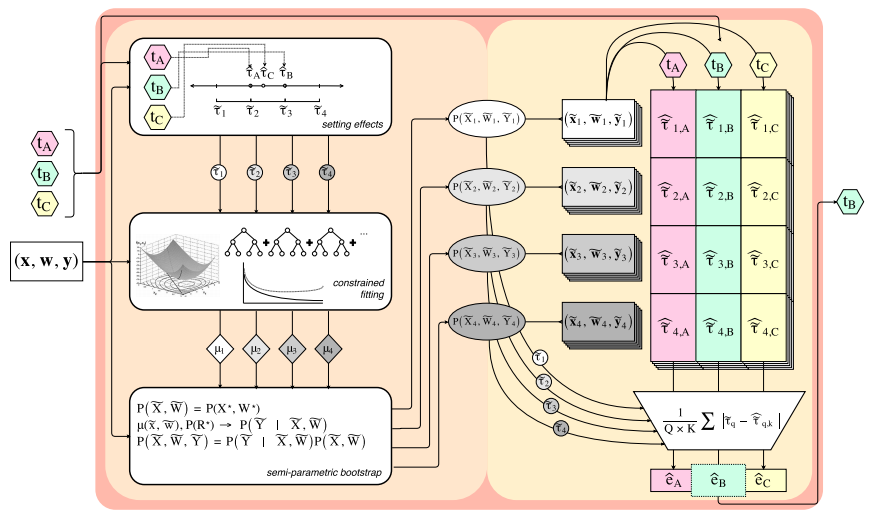
\includegraphics[height=0.5\textwidth, width=1\textwidth]{figures/synth-validation.png}
    \caption[Synth-Validation] {Synth-Validation\cite{schuler2017synth}. Die Daten $(x,w,y)$ und die Methoden für kausale Inferenz $t_A$, $t_B$ und $t_C$ kommen als Eingabe. Man wählt zuerst die synthetischen Effekte $\tau_i$, indem man die Methoden auf die Daten einsetzt. Dann schätzt man für jeden vorgegebenen synthetischen Effekt die bedingten Erwartungswerte $\mu_{0i}(x)$ und $\mu_{1i}(x)$. Man zieht eine Stichprobe von $(x,w)$ und wendet diese auf den bedingten Erwartungswerten. Somit kriegt man die synthetischen Datensätze mit einem vorgegebenen synthetischen Effekt $\tau_i$. Dann werden alle Methoden auf den Daten eingesetzt und da man den Behandlungseffekt von den Daten kennt, wird der durchschnittliche Fehler von jeder Methode ausgerechnet. Am Ende wird diejenige mit dem kleinsten Fehler ausgewählt \cite{schuler2017synth}.}\label{fig:synthValidation}
  \end{figure}
\end{center}

\noindent
In den folgenden \refsec{subsec:generierungSynthDaten} und \refsec{subsec:methodenauswahl} erzählen wir ausführlich wie die synthetischen Daten generiert werden und wie dann mit diesen neuen Daten der beste Methode für kausale Inferenz ausgewählt wird.\par

  	\subsection{Generierung von synthetischen Daten}\label{subsec:generierungSynthDaten}
  	Die generative Verteilung, die wir schätzen möchten, ist nicht die echte Verteilung $P(X,W,Y)$. Wenn man diese schätzen könnte, würden die Auswahl von den Methoden und auch die Methoden an sich umsonst, denn man könnte in diesem Fall den echten Behandlungseffekt direkt berechnen. Stattdessen wählt man zuerst synthetische Behandlungseffekten $\tilde{r_i}$. Wie genau das passiert, erzählen wir im \refsec{subsubsec:auswahlSynthEffekten}. Für unsere generativen Verteilungen  $P(\widetilde{X},\widetilde{W},\widetilde{Y})$ muss gelten, dass die davon generierten Daten maximal ähnlich zu den echten Daten sind und der durchschnittliche Behandlungseffekt von diesen Daten an unseren vorgegebenen $\tilde{r_i}$  entspricht \cite{schuler2017synth}. Formal:\par
  	
\begin{equation}\label{eq:3.1}
  \tilde{\tau} = E_{\widetilde{Y},\widetilde{X}}[\widetilde{Y}|\widetilde{X},\widetilde{W} = 1] - E_{\widetilde{Y},\widetilde{X}}[\widetilde{Y}|\widetilde{X},\widetilde{W} = 0]
\end{equation} 

\noindent
Für die Schätzung von $P(\widetilde{X},\widetilde{W},\widetilde{Y})$ benutzten wir die Beobachtung, dass $P(\widetilde{X},\widetilde{W},\widetilde{Y}) = P(\widetilde{Y}|\widetilde{X},\widetilde{W})P(\widetilde{X},\widetilde{W})$ und erstellen die beiden Verteilungen individuell. Für $P(\widetilde{X},\widetilde{W})$ nehmen wir die empirische Verteilung von $(X,W)$. Den Behandlungseffekt von \refeq{eq:3.1} kann man auch durch die von der Behandlung bedingten Erwartungswerten von $\widetilde{Y}$ darstellen\cite{schuler2017synth}:\par 

\begin{equation}\label{eq:3.2}
 \tau = \frac{1}{n}\sum_i[\mu_1(x_i)-\mu_0(x_i)]
\end{equation}

\noindent
$\mu_1(\tilde{x})$ und $\mu_0(\tilde{x})$ sind die von uns angesprochenen bedingten Erwartungswerten, indem für sie gilt:

\begin{equation}\label{eq:3.3}
\begin{split}
\mu_0(\tilde{x}) &= E[\widetilde{Y}|\widetilde{X},\widetilde{W} = 0]\\
\mu_1(\tilde{x}) &= E[\widetilde{Y}|\widetilde{X},\widetilde{W} = 1]
\end{split}
\end{equation}

\noindent
Durch die bedingten Erwartungswerten können wir ein Modell für die Generierung von $\tilde{y_i}$ erstellen:\par

\begin{equation}\label{eq:3.4}
 \tilde{y_i} = I_0(\tilde{w_i})\mu_0(\tilde{x}) + I_1(\tilde{w_i})\mu_1(\tilde{x}) + \epsilon_i
\end{equation}

\noindent
Hier ist $I_w(w_i)$ die Indikatorfunktion für die Behandlung $w_i$, indem $I_w(w_i) = 1$ für $w_i = w$ und $I_w(w_i) = 0$ für $w_i \neq w$. $\epsilon_i$ ist der Restwert von $y_i$, mit dem unsere Schätzungen von $\mu_0(\tilde{x})$ und $\mu_1(\tilde{x})$ von den echten $y_i$ abweichen. Wir müssen also zuerst die bedingten Erwartungswerten schätzen und mit deren Hilfe die Restwerten $r_i = y_i - I_0(w_i)\mu_1(x) - I_1(w_i)\mu_1(x)$ ausrechnen. Wir benutzen dann die empirische Verteilung der Restwerte $P(R^*)$ als Rauschmodell für die Schätzung von den synthetischen $\tilde{y_i}$\cite{schuler2017synth}.\par 

\noindent
Wir betonen, dass $\mu_0(\tilde{x})$ und $\mu_1(\tilde{x})$ nicht die echten bedingten Erwartungswerten von $Y$ sind, sondern die bedingten Erwartungswerten, für die $\widetilde{X}$ und $\widetilde{Y}$ aus unseren Daten kommen und für die der Behandlungseffekt $\tau$ aus \refeq{eq:3.2} an unserem vorgegebenen synthetischen Behandlungseffekt $\tilde{\tau}$ gleich ist. Wie $\mu_0(\tilde{x})$ und $\mu_1(\tilde{x})$ geschätzt werden, erzählen wir im \refsec{subsubsec:schätzungBedingtenErwartungswerten}.\par 

\noindent
Zusammenfassend geben wir die Reihenfolge von Aktionen für die Generierung von den synthetischen Daten:\par

\begin{enumerate}

\item Auswahl von synthetischen Behandlungseffekten $\tilde{\tau_1},\tilde{\tau_2}\dots$ (\ref{subsubsec:auswahlSynthEffekten}) 

\item Schätzung von den bedingten Erwartungswerten $\mu_0(\tilde{x})$ und $\mu_1(\tilde{x})$ mit den echten Daten $(x_i,w_i,y_i)$ und den ausgewählten synthetischen Behandlungseffekten $\tilde{\tau_1},\tilde{\tau_2}\dots$ aus Schritt 1  (\ref{subsubsec:schätzungBedingtenErwartungswerten})

\item Stichprobeziehen aus den echten Daten $(x_i,w_i)$ für die Generierten $(\tilde{x_i},\tilde{w_i})$ 

\item Einsetzen von $(\tilde{x_i},\tilde{w_i})$ aus Schritt 3 in $\mu_0(\tilde{x})$ und $\mu_1(\tilde{x})$ aus Schritt 2 für die Schätzung von den Ergebnissen ohne Restwerte

\item Ausrechnung von den Restwerten $r_i$ durch $y_i$ und die Ergebnisse aus Schritt 4; Stichprobeziehen aus den ausgerechneten Restwerten $r_i$ für $\tilde{r_i}$

\item Generierung von $\tilde{y_i}$ durch Addieren von den Ergebnissen aus Schritt 4 mit den gezogenen Restwerten $\tilde{r_i}$ aus Schritt 5

\end{enumerate}
  		\subsubsection{Auswahl von synthetischen Effekten}\label{subsubsec:auswahlSynthEffekten}
  		Damit man die vorhandenen Methoden für kausale Inferenz auf Daten mit bekannten Behandlungseffekten testen kann, muss man zuerst diese Effekten bestimmen. Sie müssen so nah wie möglich an dem echten Behandlungseffekt liegen, damit die Auswahl am Ende sinnvoll ist. Die besten Schätzungen für ihn kriegt man durch den Einsatz von den Methoden. Es ist unklar, welche die Beste ist, deswegen benutzt man eine Heuristik\cite{schuler2017synth}.\par 
  		
\noindent
Die Anzahl aller synthetischen Effekten $Q$ und ein Parameter $\gamma$ kommen als Eingabe, indem wir $Q=5$ und $\gamma = 2$ in unserer Implementierung benutzen. Man führt zuerst jede Methode $t$ auf den Daten aus und kriegt die Schätzungen $\hat{\tau_t}$. Dann wird die Median von allen Schätzungen gefunden. Den kleinsten synthetischen Effekt bestimmt man, indem von der Median der Produkt von der Spannweite $R$ aller Schätzungen und dem Parameter $\gamma$ abgezogen wird. Der größte synthetische Effekt ist die Summe von der Median und dieses Produkt. Für den Rest der Effekten nimmt man die Werte, die auf gleichen Intervallen in dieser Spannweite liegen, sodass alle Effekte insgesamt $Q$ sind\cite{schuler2017synth}.

\begin{equation}\label{eq:3.5}
\begin{split}
 \tilde{\tau_1} &= med(\hat{\tau_t}) - \gamma R\\
 \tilde{\tau_Q} &= med(\hat{\tau_t}) + \gamma R
\end{split}
\end{equation}
	
\subsubsection{Schätzung von bedingten Erwartungswerten}\label{subsubsec:schätzungBedingtenErwartungswerten}
Wir müssen die bedingten Erwartungswerten $\mu_0(\tilde{x})$ und $\mu_1(\tilde{x})$ schätzen. Es lohnt sich, noch einmal zu wiederholen, dass sie nicht die echten bedingten Erwartungswerten, sondern diejenige, für die unsere Daten einen vorgegebenen Behandlungseffekt $\tilde{\tau}$ haben. Für die Schätzung soll man das folgende Problem lösen\cite{schuler2017synth}:\par

\begin{equation}\label{eq:3.6}
\begin{split}
 \mu_0(\tilde{x}),\mu_1(\tilde{x}) = &\arg\min_{f_0,f_1 \in F} \quad \sum_{S_0} l(y_i,f_0(x_i)) + \sum_{S_1} l(y_i,f_1(x_i))\\
 &\text{bedingt von: } \frac{1}{n} \sum_i \big [f_1(x_i) - f_0(x_i) \big ] = \tilde{\tau}
\end{split}
\end{equation}

\noindent
Hier ist $l(y_i,f)$  eine Verlustfunktion z.B. $(y-f)^2$. Für die Lösung des Problem wird Constrained Gradient Boosting eingesetzt. Constrained Boosting ist eine Form von Gradient Boosting (\ref{subsubsubsec:gradientBoosting}), die aber eine Nebenbedingung für die geschätzten Funktionen hat. Im Folgenden werden wir das Algorithmus von Constrained Boosting darstellen\cite{schuler2017synth}.\par
 
\noindent
Man versucht, die bedingten Erwartungswerten als Summe von vielen Basisfunktionen $b_{w_j}(\tilde{x})$ zu berechnen. Formal:\par

\begin{equation}\label{eq:3.7}
 \mu_{w_m}(\tilde{x}) = \sum_j^m \upsilon_{w_j}b_{w_j}(\tilde{x})
\end{equation}

\noindent
Man schätzt die Basisfunktionen in jedem Schritt neu und addiert sie zu dem bisherigen Schätzwert. Die ersten Schätzwerten $b_{0_1}$ und $b_{1_1}$ sind Konstanten und es gilt $\upsilon_{0_1} = \upsilon_{1_1} = 1$. Wir finden sie durch die Lösung vom folgenden Problem\cite{schuler2017synth}: \par 

\begin{equation}\label{eq:3.8}
\begin{split}
	\mu_{0_1}(\tilde{x}),\mu_{1_1}(\tilde{x}) = b_{0_1},b_{1_1} = &\arg\min_{c_0,c_1} \quad \sum_{S_0} l(y_i,c_0) + \sum_{S_1} l(y_i,c_1)\\
 &\text{bedingt von: } \tilde{\tau} = \frac{1}{n} \sum_i \big [c_1 - c_0 \big ]
\end{split}
\end{equation}

\noindent
In den weiteren Schritten $m>1$ nimmt man die Restwerte $r_{{m-1}_i}$ von der letzten Schätzung $\mu_{w_m}(x_i)$ und $y_i$ und passt die Basisfunktionen $b_{w_m}(x)$ zu ihnen an. Dafür wird ein Regressionsbaum benutzt. In \refeq{eq:3.9} ist $I_w(w_i)$ die Indikatorfunktion für die Behandlung $w_i$ \cite{schuler2017synth}. Formal:\par

\begin{equation}\label{eq:3.9}
r_{{m-1}_i} = y_i - I_0(w_i)\mu_{0_{m-1}}(x_i)-I_1(w_i)\mu_{1_{m-1}}(x_i)
\end{equation}

\begin{equation}\label{eq:3.10}
\begin{split}
	 b_{0_m}(x) = &\arg\min_{b \in B} \sum_{S_0} l(r_{{m-1}_i},b(x_i))\\
	 b_{1_m}(x) = &\arg\min_{b \in B} \sum_{S_1} l(r_{{m-1}_i},b(x_i))
\end{split}
\end{equation}

\noindent
Man merkt, dass die Anpassung von den Basisfunktionen ohne die Bedingung über den synthetischen Behandlungseffekt stattfindet. Aus diesem Grund darf man nicht direkt $\mu_{w_{m-1}}(x_i)$ mit $b_{w_m}(x)$ addieren. Wir suchen deswegen nach den Koeffizienten $\upsilon_{0_m}$ und $\upsilon_{1_m}$, für die der Behandlungseffekt $\tilde{\tau}$ bleibt. Die Bedingung ist im ersten Schritt erfüllt. Soweit der Beitrag zu dem Behandlungseffekt in jedem weiteren Schritt $0$ ist, bleibt die Bedingung erfüllt\cite{schuler2017synth}. Deswegen lösen wir das Optimierungsproblem:\par 

\begin{equation}\label{eq:3.11}
\begin{split}
	\upsilon_{0_m},\upsilon_{1_m} = \arg\min_{c_0,c_1} \quad &\sum_{i \in S_0} l \big (y_i,\mu_{0_{m-1}}(x_i) + c_0  b_{{0_i}_m}(x_i) \big ) + \lambda c_0^2 + \\
 &\sum_{i \in S_1} l \big (y_i,\mu_{1_{m-1}}(x_i) + c_1  b_{{1_i}_m}(x_i) \big ) + \lambda c_0^2\\
  \text{bedingt}& \text{ von: } \sum_i \big [c_1 b_{{1_i}_m}(x_i) - c_0 b_{{0_i}_m}(x_i) \big ] = 0
\end{split}
\end{equation}
  	
\noindent
 $\lambda$ dient zur Regulierung von der Schätzung, sodass sie weniger Varianz hat. Am Ende berechnet man die $\mu_{0_m}(\tilde{x})$ und $\mu_{1_m}(\tilde{x})$ durch \refeq{eq:3.7}. Die Anzahl von Schritten $m$ ist von Anfang an nicht bekannt. Wenn sie zu niedrig ist, wird die Schätzung viel Bias haben. Wenn zu hoch, zu viel Varianz. Deswegen wird die optimale $m$ durch Cross-Validation bestimmt\cite{schuler2017synth}.\par
    	
\subsection{Methodenauswahl}\label{subsec:methodenauswahl}

Nachdem man die generativen Verteilungen geschätzt hat, kann man synthetische Daten mit bekannten Behandlungseffekten generieren und die Methoden darauf ausführen. Von jeder Verteilung generiert man $K$ Stichproben, was für die $Q$ Verteilungen  insgesamt $Q \times K$ Datensätze $d_{q,k}$ macht. Jeder Methode $t$ wird auf jeden Datensatz $d_{q,k}$ ausgeführt, was insgesamt  $T \times Q \times K$ Schätzungen $\hat{\tilde{\tau}}_{t,q,k}$ von dem synthetischen Behandlungseffekt erzeugt. Es wird dann den absoluten Fehler $\tilde{e_{t,q,k}} = |\tilde{\tau}_q - \hat{\tilde{\tau}}_{t,q,k}|$ von jeder Schätzung  ausgerechnet. Zum Schluss rechnet man den durchschnittlichen Fehler $e_t$ für jede Methode und wählt die Methode mit dem kleinsten Fehler\cite{schuler2017synth}:\par

\begin{equation}\label{eq:3.12}
 t^{\times} = \arg\min_{t \in T} \sum_{q,k}^{Q,K} \tilde{e}_{t,q,k}
\end{equation}
\clearpage

\section{Implementierung}\label{sec:implementierung}
\noindent
\emph{In diesem Abschnitt erzählen wir über unsere Implementierung. Wir erläutern zuerst, was wir genau programmiert haben, welche Technologien wir benutzt haben und warum und stellen einige allgemeinen Angaben bereit. Dann gehen wir konkret durch die einzelnen Bestandteile der Implementierung durch und erläutern, wozu sie dienen, welche Algorithmen und Techniken wir benutzt haben und wie sich die Theorie aus den vorigen Abschnitten in der Implementierung abbildet.}\par

Wir haben Synth-Validation\cite{schuler2017synth} implementiert - ein Auswahlverfahren von Methoden für kausale Inferenz, über den wir im vorigen \refsec{sec:synthValidation} erzählt haben. Den Code kann man unter \url{https://github.com/naskoD/bachelorThesis} frei zugreifen. Wir haben einen wesentlichen Teil des Codes von den Autoren von Synth-Validation bekommen. Er war auf Julia geschrieben und wir haben diesen Code direkt mit winzigen Logikänderungen in R übersetzt. In den Unterabschnitten werden wir für die einzelnen Bestandteilen bezeichnen, ob sie übersetzt sind oder rein von uns kommen.\par 

\noindent
Die Implementierung hat sich aufwändiger als erwartet erwiesen. Am Ende sind wir mit insgesamt 1650 Codezeilen ohne die Tests und 2200 mit den Tests gekommen. Sie sind in 13 Skripte ohne die Tests und 19 mit den Tests verteilt. Wir könnten wegen Zeitmangel und Streben nach Effizienz nicht alle Bestandteile mit Unittests überdecken. Wenn wir auch die Scripte von unseren Experimenten in der Rechnung hinzufügen, wo wir Synth-Validation mit unterschiedlichen Daten und unter unterschiedlichen Bedingungen benchmarken, kommen wir zu insgesamt 2350 Codezeilen in 25 Scripten.\par 

\noindent
Wir haben R für die Implementierung gewählt, weil diese Scriptsprache sich als Standard für statistikbezogene Projekten durchgesetzt hat. Es gibt eine große Anzahl von fertigen Bibliotheken, die zur Verfügung stehen. Außerdem hat sie einen intuitiven Syntax, der eine schnelle Implementierung erlaubt. Die Sprache wird von vielen Wissenschaftler und Praktiker benutzt und in den seltenen Fällen, in denen eine Bibliothek nicht ausreichend oder gar nicht dokumentiert ist, kann man schnell Unterstützung im Netz finden. R hat natürlich Nachteile -  z.B die niedrigere Geschwindigkeit im Vergleich zu anderen Alternativen wie Python oder Julia. Mehr darüber erzählen wir im \refsec{subsec:methodikDaten}, wo wir unter anderem auch Daten über die Performance von der Implementierung geben.\par    

\subsection{Externe Paketen}\label{subsec:externePaketen}

\noindent
\emph{In diesem Abschnitt erzählen wir über die externen Paketen, die wir in unserer Implementierung benutzt haben. Wir werden sie in der Reihe des Auftretens im Programm vorstellen.}\par

\noindent
Das erste Paket ist \textbf{tictoc}. Es dient zur Zeitbemessung bei der Ausführung von einem Script oder einem Codeteil. Da ein Lauf von Synth-Validation sogar mit Standardparameter relativ lange dauert, ist es sinnvoll zu wissen, wie viel Zeit jeder einzelnen Bestandteil braucht. Das gilt sowohl für die Zeit während des Laufs, als auch für die Analyse nach dem Ende. Dementsprechend ist ein Code aus dem Paket an vielen Stellen in unserer Implementierung vertreten.
\par

\noindent
Ein weiteres Paket, dessen Code man oft in unserer Implementierung trifft, ist \textbf{assertthat}. Es dient zur Validierung von Argumenten und ist in fast jeder Funktion unseres Codes zu finden.
\par

\noindent
Aus dem Paket \textbf{psych} benutzen wir einmalig die logistische Funktion.\par 

\noindent
An mehreren Stellen (z.B intern in unseren Datenstrukturen und in der Logik von Constrained Boosting) benutzen wir Dictionaries, die wir aus dem Packet \textbf{collections} nehmen. Meistens hat die Dictionary zwei Schlüssel für behandelt und unbehandelt und die Werte sind Arrays mit unterschiedlichen Daten.\par

\noindent
Wir nutzen einmalig die Funktion \emph{fold} aus dem Paket \textbf{mltools} bei der Cross-Validation, die die optimale Anzahl von Schritten für Constrained Boosting feststellt. \emph{fold} teilt den Datensatz auf Training- und Testdata nach bestimmten Kriterien. Ansonsten enthält das Paket Hilfefunktionen, die man in Techniken aus dem maschinellen Lernen benutzt.\par 
 
\noindent
Durch Funktionen aus dem Paket \textbf{NlcOptim} kann man Optimierungsproblemen lösen. Wir brauchen es bei der Bestimmung von den Koeffizienten $\upsilon_{0_m}$ und $\upsilon_{1_m}$ für die geschätzten Basisfunktionen in Constrained Boosting.\par 
 
\noindent
Das Paket \textbf{devtools} dient zur Arbeit mit Paketen z.B. Entwicklung, Installierung, usw. Wir benutzen es, um das Paket \textbf{rlearner} direkt aus Github zu installieren.\par

\noindent
Mit \textbf{gridExtra} kann man Grids mit Daten schön stilisieren und dann generieren. Wir benutzen es einmal bei der Erstellung von Abbildungen für die Erfolgsrate von Synth-Validation.\par

\noindent
Mit dem Paket \textbf{testthat} erstellt man Unittests. Wir haben 6 Testskripten, die es benutzen.\par

\noindent
Vielleicht die wichtigsten externen Paketen, die wir nutzen, sind \textbf{rlearner} und \textbf{grf}. Sie beinhalten die Schätzer von den Methoden für kausale Inferenz, von denen Synth-Validation wählt. Wir haben die Theorie dahinter im \refsec{subsec:methodenInImplementierung} erläutert. \textbf{rlearner} hat den Quasi-Orakel Schätzer mit Gradient Boosting und Lasso und  \textbf{grf} hat die kausale Wälder. Wir benutzen die Funktionen aus diesen Paketen in unseren Wrapper-Funktionen, die die getestete Methoden für kausale Inferenz darstellen.\par
\subsection{Lesen/Schreiben von Daten}\label{subsec:lesenSchreibenDaten}

\noindent
Im Script \textbf{read\_write\_data.r} haben wir Funktionen implementiert, die sich um das Lesen und Schreiben von Daten in Dateien kümmern. Wir haben sie selbst entwickelt und nicht aus dem Juliacode übersetzt. Grundsätzlich lesen wir unsere Daten aus .csv Dateien und schreiben dann die Ergebnisse aus dem Benchmark wieder in .csv Dateien. Ab dem Moment, in dem wir angefangen haben, Analyseszenarien für die Evaluation auszudenken, haben wir festgestellt, dass es sehr nützlich wäre, wenn wir ein kleines Datenbank eingesetzt hätten. Die Zeit war aber für solche Änderungen knapp, deswegen sind wir mit der einfachen .csv Abspeicherung geblieben.\par 

\noindent
Wir haben unterschiedlichen Datenquellen, deren Daten ein unterschiedliches Format hatten, deswegen war die erste Aufgabe, die Daten zu normalisieren. Dann war der echte Behandlungseffekt von einigen Datensätzen nicht direkt gegeben und man sollte ihn aus den echten bedingten Erwartungswerten ausrechnen und in einer Datei abspeichern. Das waren die beiden Vorbereitungsschritten, die wir durchgeführt haben und deren Code im Lauf von Synth-Validation nicht läuft. Dann haben wir Funktionen für das Lesen von den Eingabedaten (Kovariaten, Behandlung, Ergebnisvariable und echten Behandlungseffekt). Weitere Funktionen dienen zum Lesen und Schreiben von Benchmarkdaten. Wenn es einen neuen Dateneintrag gibt, lesen wir zuerst die vorhandenen Daten, fügen ihn dazu ein und speichern alles zusammen. Wir haben eine Funktion, die den normalen Lauf des Programms sichert, indem sie die die Verzeichnisstruktur der Benchmarkdaten neu erstellt, wenn das Programm zum ersten Mal läuft oder wenn man sie gelöscht hat.\par

\subsection{Ziehen von Stichproben}\label{subsec:ziehenStichproben}
Das Ziehen von Stichproben spielt eine sehr wichtige Rolle in unserer Implementierung. Aus den Daten, die wir gelesen haben, nehmen wir für die Schätzung nicht alle, sondern nur einen Teil davon (Standardwert ist 100). So simulieren wir eine echte Beobachtungsstudie, in der man nicht alle Objekte aus der Grundgesamtheit beobachtet, weil das oft unmöglich ist. Wir kennen den durchschnittlichen Behandlungseffekt von allen Beobachtungen und analysieren nur einen Teil davon. So stellen wir die ganze Datenmenge als die Grundgesamtheit, obwohl sie keine echte Grundgesamtheit ist, über die wir den echten Behandlungseffekt kennen. In einem Experiment im \refsec{sec:ergebnisseEvaluation} bemessen wir die Auswirkung von der Anzahl der analysierten Objekten auf die Schätzung von Synth-Validation.\par

\noindent
Wir ziehen Stichproben an noch einer Stelle in der Implementierung und zwar bei der Generierung von synthetischen Daten. Nachdem wir die bedingte Erwartungswerte durch Constrained Boosting geschätzt haben und die entsprechenden Restwerte ausgerechnet haben, ziehen wir $2k$ Stichproben mit Zurücklegen mit der gleichen Anzahl von Elementen für die $k$ synthetischen Datensätze. Es gibt also zwei unabhängige Stichproben für jeden Datensatz - die Erste für die $(\tilde{x_i},\tilde{w_i})$, deren Werte wir dann in den geschätzten bedingten Erwartungswerten einsetzen und die Zweite für die Restwerte, die wir dann mit den vorigen Ergebnissen addieren und die fertigen synthetischen $\tilde{y_i}$ bekommen. Dieser Codebestandteil haben wir auch nicht aus den Juliacode übersetzt, sondern selbst implementiert. Die Logik befindet sich im Script \textbf{sampling.r}.
  	\subsection{Methoden für kausale Inferenz}\label{subsec:methodenKausaleInferenz}
  	In unserer Implementierung wählt  Synth-Validation aus vier Methoden für kausale Inferenz - die naive Methode, Quasi-Orakel Schätzer mit Gradient Boosting, Quasi-Orakel Schätzer mit Lasso und Kausale Wälder. Wir haben sie außer der naiven Methode nicht selber implementiert, sondern aus den Paketen \textbf{rlearner} und  \textbf{grf} genommen. Wie schon mal im \refsec{subsec:methodenInImplementierung} angesprochen, schätzen die drei Methoden den heterogenen Behandlungseffekt. Deswegen haben wir in \textbf{causal\_inference\_methods.r} für jede Methode eine Wrapperfunktion geschrieben, in der wir den durchschnittlichen Behandlungseffekt aus allen heterogenen Schätzungen ausrechnen. Wir führen die Methoden an zwei Stellen in der Implementierung aus - einmal am Anfang auf den echten Daten, um die synthetischen Effekten zu bestimmen und einmal auf jeden generierten synthetischen Datensatz. \par
\subsection{Synth-Validation}\label{subsec:synthValidation}
\noindent
\emph{Alle in diesem Abschnitt beschriebenen Codebestandteile (ohne diese im  \emph{\hyperref[subsubsec:methodenauswahl]{Unterabschnitt Methodenauswahl}} haben wir nicht selber entworfen, sondern aus dem Juliacode von den Autoren in R übersetzt.} \par
\subsubsection{Datenstrukturen}\label{subsubsec:datenstrukturen}

Wir könnten für unsere Implementierung nur die einfachen Listen und Vektoren benutzen. So eine Entscheidung würde aber den Code unnötig kompliziert und unleserlich machen. Deswegen haben wir die Datenstrukturen genommen, die im Juliacode waren. Das sind nämlich die Klassen \textbf{Data}, \textbf{Counterfactuals}, \textbf{TreatmentDictionary}, \textbf{NumericTreatmentDictionary} und \textbf{Synth\_Validation\_Result}, die sich im Script \textbf{data\_structures.r} befinden.\par 

\noindent
Die Klasse \textbf{Data} enthält  eine Matrix $X$ für die Kovariaten, einen logischen Vektor $W$ für die Behandlung und einen Vektor $Y$ für die Ergebnisvaeiable. Wir benutzen die Klasse sowohl für die echten, als auch für die synthetischen Daten.\par 

\noindent
Ein Objekt aus der Klasse \textbf{Counterfactuals} ist das Ergebnis aus einem Schritt von Constrained Boosting. Es enthält die bedingten Erwartungswerten für alle Elementen aus \textbf{Data}.\par 

\noindent
\textbf{TreatmentDictionary} hat für die beiden Schlüssel \emph{behandelt} und \emph{unbehandelt} einen Vektor mit irgendwelchen Elementen. Wir benutzen es bei der Schätzung, wo die Elemente z.B. angepasste Regressionsbäume sind.\par	

\noindent
\textbf{NumericTreatmentDictionary} ist wie \textbf{TreatmentDictionary}, aber seine Elementen dürfen nur numerisch sein. Wir benutzen sie an mehreren Stellen. Ein Objekt aus dieser Klasse ist z.B. das Ergebnis von den Schätzungen der Basisfunktionen bei Constrained Boosting.\par

\noindent
Die letzte datenbezogene Klasse ist \textbf{Synth\_Validation\_Result} und sie trägt das Ergebnis von Synth-Validation. Wir haben sie selbst entwickelt. Die Klasse enthält drei Felder - der Index der ausgewählten Methode, die Schätzung dieser Methode und ein Vektor mit den Schätzungen von allen Methoden. Wir benutzen sie beim Benchmark. \par

\subsubsection{Schätzung}\label{subsubsec:schätung}
Im Skript \textbf{estimators.r} haben wir den Regressionsbaum implementiert, den wir im Juliacode gefunden habe. Er schätzt die Basisfunktionen im Constrained Boosting, wobei er die Restwerte von $y_i$ und der vorigen Schätzung nimmt. Wir setzen die minimale Anzahl von Elementen im Blatt auf fünf und die maximale Tiefe des Baums auf drei. Hier haben wir eine winzige Änderung in der Logik des Baums im Vergleich zu dieser im Juliacode - wir haben einen Sonderfall beim Aufspalten behoben, indem wir nicht aufspalten, wenn das maximale MSE null ist und alle $Y$ gleich sind.\par

\subsubsection{Constrained Boosting}\label{subsubsec:constrainedBoosting}

Das Constrained Gradient Boosting Algorithmus und die Cross-Validation dazu implementieren wir im Script \textbf{constrained\_boosting.r}. Grundsätzlich machen wir das, was wir im \refsec{subsubsec:schätzungBedingtenErwartungswerten} theoretisch beschrieben haben. Im ersten Schritt finden wir die beiden Konstanten für die bedingten Erwartungswerten und berechnen die Restwerte für jedes Element. Dann fängt eine Schleife an, wobei jeder Lauf einen weiteren Schritt aus dem Constrained Boosting ist. Im jedem Lauf passen wir zuerst den Regressionbaum für die Schätzung der Basisfunktionen an. Dann erstellen wir eine Dictionaty, die als Schlüssel die einzigartigen Schätzungen des Baums hat. Die Werte für die Schlüssel sind dann die Indexen von den Elementen, die diese Schätzung haben. Wir nehmen dann diese Dictionaty und benutzen sie in unser Optimierungsproblem, indem wir den allgemeinen Verlust als die Summe von den Verlusten von alle einzigartigen Schätzungen und den Verlust von einer einzigartigen Schätzung als die Summe von den Verlusten von den Elementen mit dieser Schätzung. Für das Optimierungsproblem benutzen wir das externe Paket \textbf{NlcOptim} und finden die Ko­ef­fi­zi­enten, für die unsere Bedingung hält. Dann addieren wir die Basisfunktion mit seinen Koeffizienten zu der alten Schätzung und bekommen die neuen bedingten Erwartungswerten.\par 

\noindent
Bevor wir Constrained Boosting produktiv einsetzen, müssen wir die optimale Anzahl von Schritten bestimmen, sodass die MSE der Schätzung minimal ist. Dazu benutzen wir Cross-Validation. Wir teilen die Daten auf Training- und Testdaten. Dann führen wir Constrained Boosting auf den Trainingdaten mit der Ausnahme, dass wir für die Bedingung über den synthetischen Effekt im Optimierungsproblem alle Daten benutzen. Dann messen wir den Schätzfehler in jedem Schritt mit den Testdaten. Wir wiederholen das vier mal und wählen als Anzahl die Nummer des Schritts mit dem kleinsten durchschnittlichen Testfehler für diese vier Läufe.\par  

\subsubsection{Methodenauswahl}\label{subsubsec:methodenauswahl}
Die Methodenauswahl findet in der Methode \emph{pick\_best\_method} im Skript \textbf{synth-validation.r} statt. Wir haben sie selber implementiert. Sie nimmt als Argumenten die synthetischen Datensätze und die synthetischen Effekte. Dann führt sie die Methoden für kausale Inferenz auf den Daten aus, bemesst ihren durchschnittlichen Fehler als absoluten Abstand der Schätzung von dem synthetischen Effekt und wählt die Methode mit dem kleinsten Fehler aus.\par 
  	\subsection{Benchmark von Synth-Validation}\label{subsec:benchmarkSynthValidation}
Durch den Benchmark prüfen wir, wie die Schätzungen von Synth-Validation im Vergleich zu den Schätzungen von den anderen Methoden verhalten. Das Maß, die wir nutzen, ist der absolute Fehler von dem echten durchschnittlichen Behandlungseffekt. Aus diesem Grund müssen wir ihn vorher kennen. Wir führen also mehrmals ($n>30$) die Synth-Validation mit gleichen Daten und gleichen Paramerter aus und vergleichen ihren durchschnittlichen Fehler mit den durchschnittlichen Fehlern der Methoden. Noch beobachten wir nebeneinander, wie oft eine Methode die Orakel-Schätzung (die beste Schätzung unter allen Methoden) hat und wie oft sie von Synth-Validation ausgewählt wird. Die Orakel-Schätzung kann für einen bestimmten Datensatz unterschiedlich sein, da wir bei jedem Lauf von Synth-Validation immer eine neue Stichprobe aus diesem gleichen, viel größeren Datensatz (unsere Grundgesamtheit) ziehen. Wir beobachten noch, wie erfolgreich Synth-Validation auswählt. Das machen wir im Sinne davon, wie oft die Schätzung von Synth-Validation mit der besten Schätzung (Orakel-Schätzung), mit der zweitbesten usw übereinstimmt. Diese Analysen führen wir auf unterschiedlichen Ebenen - für einen bestimmten Datensatz, für alle Datensätze aus einer Art und für insgesamt alle Datensätze.\par 

\noindent
Im Skript \textbf{synth\_validation\_benchmark.r} haben wir die Struktur von dem Benchmark aufgebaut - wir rufen Funktionen aus anderen Skripten, die die Arbeit erledigen. Da berechnen wir natürlich den absoluten Fehler der Schätzungen aus einem Lauf und leiten ihn zum Speichen und zum Erstellen von Abbildungen weiter. Im Skript \textbf{benchmark\_analysis.r} machen wir die Berechnungen für die im oberen Paragraf beschriebenen Analysen. \par 

\subsection{Erstellung von Abbildungen}\label{subsec:erstellungAbbildungen}

Wir nehmen die Daten aus den Skripten \textbf{benchmark\_analysis.r} und \textbf{synth\_\\validation\_benchmark.r} und erstellen damit im Skript \textbf{plots.r} Abbildungen für unsere Analyse. Es gibt drei Arten, die wir generieren - ein Boxplot, der den Schätzfehler von Synth-Validation und allen Methoden zeigt, ein Balkendiagramm, der die Häufigkeit von der Auswahl jeder Methode aus dem Orakel und aus Synth-Validation zeigt und eine Tabelle, die die kumulative Erfolgsrate von Synth-Validation zeigt. Dazu benutzen wir keine externen Pakete, sondern nur die Standardfunktionen in R. Man kann die drei Abbildungsarten im \refsec{sec:ergebnisseEvaluation} oder im \emph{\hyperref[anhang]{Anhang}} anschauen. 


\subsection{Experimenten}\label{subsec:experimenten}
In unserer Evaluation wollen wir unterschiedliche Szenarien testen - wie stellt sich Synth-Validation mit unterschiedlichen Daten, mit einer unterschiedlichen Größe der gezogenen Stichprobe und mit einer unterschiedlichen Anzahl von der maximalen Schritten bei Constrained Boosting vor. Die sechs Skripte der Experimente \textbf{experiments*.r} enthalten ausschließlich Aufrufe von der Funktion \emph{benchmark} aus dem Skript \textbf{synth\_validation\_benchmark.r} mit unterschiedlichen Konfigurationsargumenten. Wir stellen die Ergebnisse aus den Experimenten im \refsec{sec:ergebnisseEvaluation} dar.\par

\subsection{Unittests}\label{subsec:unitTests}
Wir haben Unittests für die Funktionen aus den Skripten von Synth-Validation geschrieben. Dafür haben wir das externe Paket \textbf{testthat} benutzt. Die Unittest haben keinen besonders großen Nutzen gebracht, aber ihre Entwicklung und vor allem Wartung kosteten Zeit. Und da wir mit unserer Arbeit Effizienz anstreben und die Zeit knapp war, haben wir für den Rest der Implementierung nur manuell getestet.\par 
      	  	
\subsection{Anderer Code}\label{subsec:andererCode}
Wir haben das Skript \textbf{install\_required\_packages.r} geschrieben, das in jedem Experiment als erstes gerufen wird. Er prüft, ob die notwendigen externen Paketen installiert sind und wenn nicht, installiert sie. Im Skript \textbf{utilities.r} haben wir einige allgemein nützliche Funktionen implementiert, die wir an vielen Stellen in der Implementierung nutzen. Eine davon ist z.B. \emph{assert\_integer}.   

\clearpage

\section{Ergebnisse und Evaluation}\label{sec:ergebnisseEvaluation}
  	\subsection{Methodik und Daten}\label{subsec:methodikDaten}
  	\subsection{TODO}\label{subsec:todo} %TODO
\clearpage

\section{Schlussfolgerung}\label{sec:schlussfolgerung}
  	\subsection{Zusammenfassung}\label{subsec:zusammenfassung}
  	\subsection{Diskussion}\label{subsec:diskussion}
\clearpage
	
%main content ends here

\begin{interlude}
  
  \begin{appendices}
  \label{anhang}
   
  \end{appendices}
  \clearpage
  \addcontentsline{toc}{section}{Literatur}
  \bibliographystyle{alpha}
  \bibliography{references}
\end{interlude}
\end{document}


